\section{Этикет и правила поведения}

В данном разделе описываются общепринятые правила поведения и этикета, которые позволяют играть более быстро и ясно, делать меньше ошибок и провоцировать меньше спорных ситуаций. Мы рекомендуем придерживаться этих правил в любой игре --- ваши оппоненты будут вам благодарны. О потенциальных последствиях несоблюдения рекомендаций будет написано отдельно в каждом пункте, кроме того можно также заглянуть в раздел о судейских регламентах для уточнений.

Основные рекомендации в процессе игры --- с одной стороны не спешить и успевать делать все четко, с другой --- не затягивать раздачу. 

\newpage

\subsection {Начало игры}

Перед началом игры игроки должны тщательно перемешать тайлы. Рекомендуемый порядок перемешивания таков:

\begin{itemize}
	\item Тщательно перемешать тайлы, игнорируя переворачивающиеся тайлы в процессе перемешивания
	\item Перевернуть все тайлы рубашкой вверх
	\item Осторожно перемешать тайлы еще раз, стараясь их не переворачивать. Хороший способ - водить руками по столу и толкать тайлы ("гладить стол"). Если какие-то из тайлов перевернулись, их следует немедленно перевернуть обратно.
\end{itemize}

\begin{figure}[H]
	\centering
	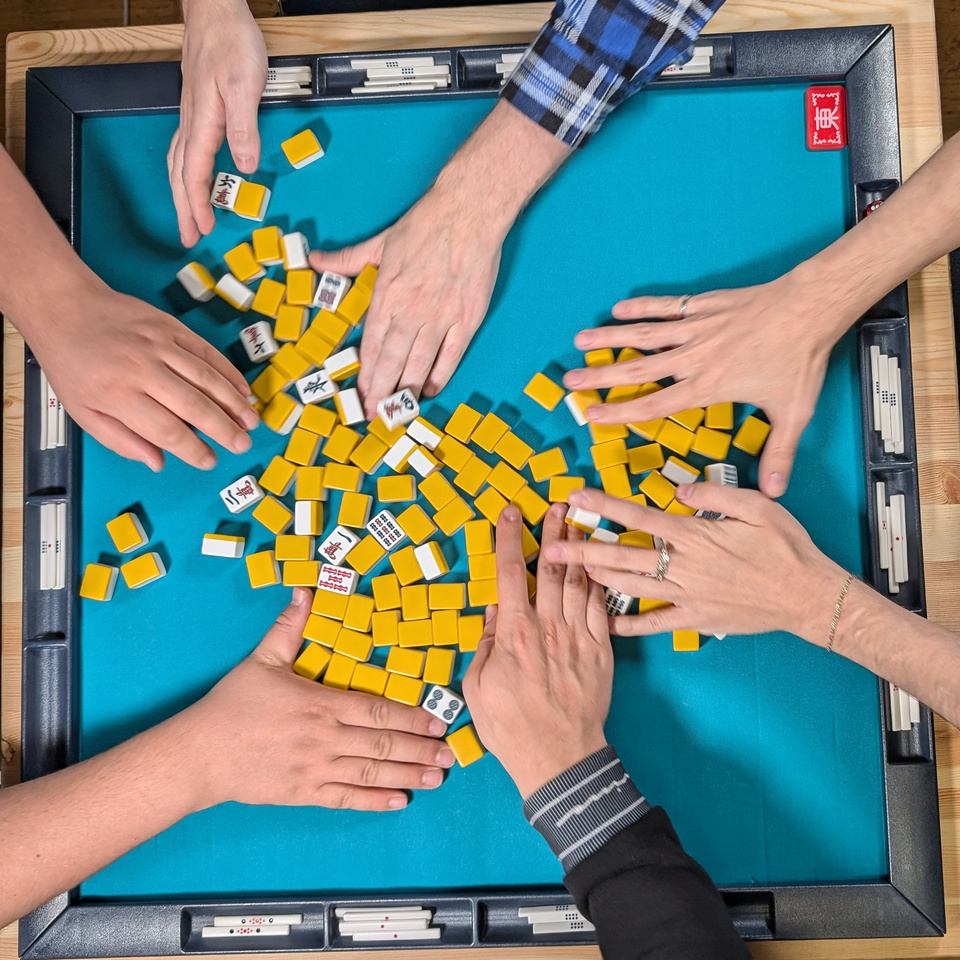
\includegraphics[width=8cm]{01_shuffle.jpg}
	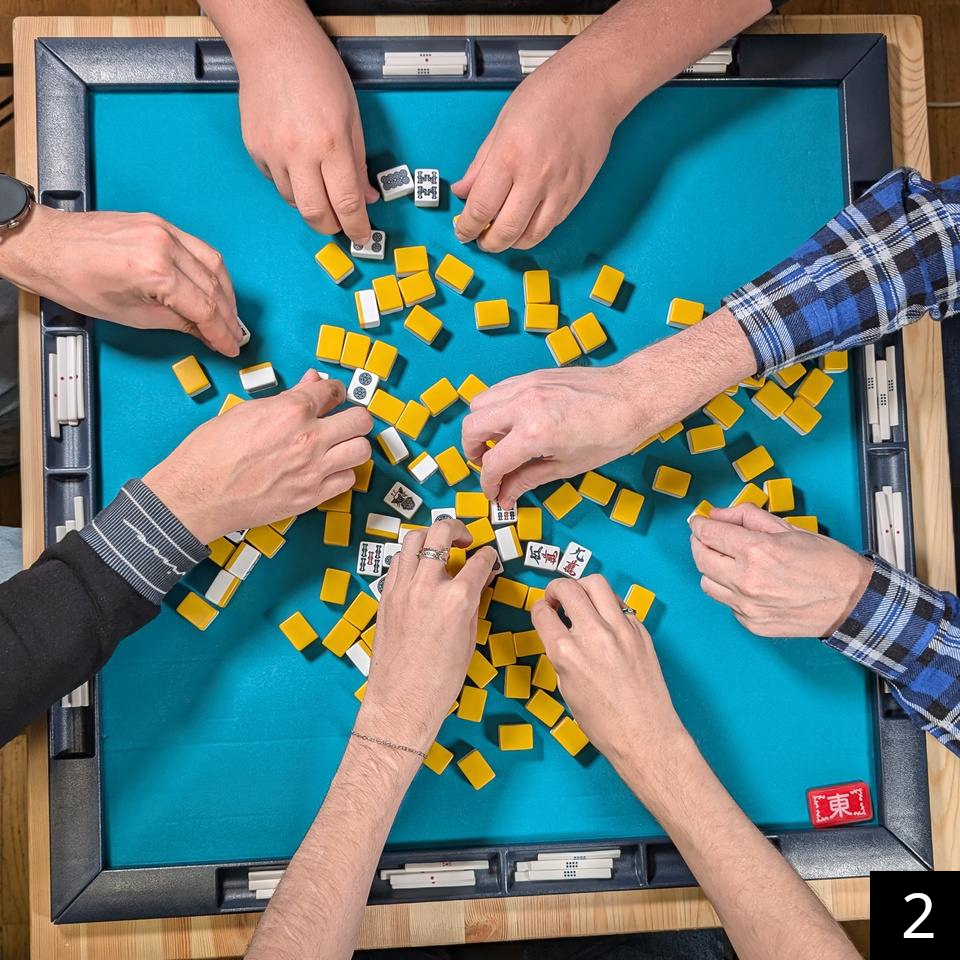
\includegraphics[width=8cm]{02_shuffle.jpg}
	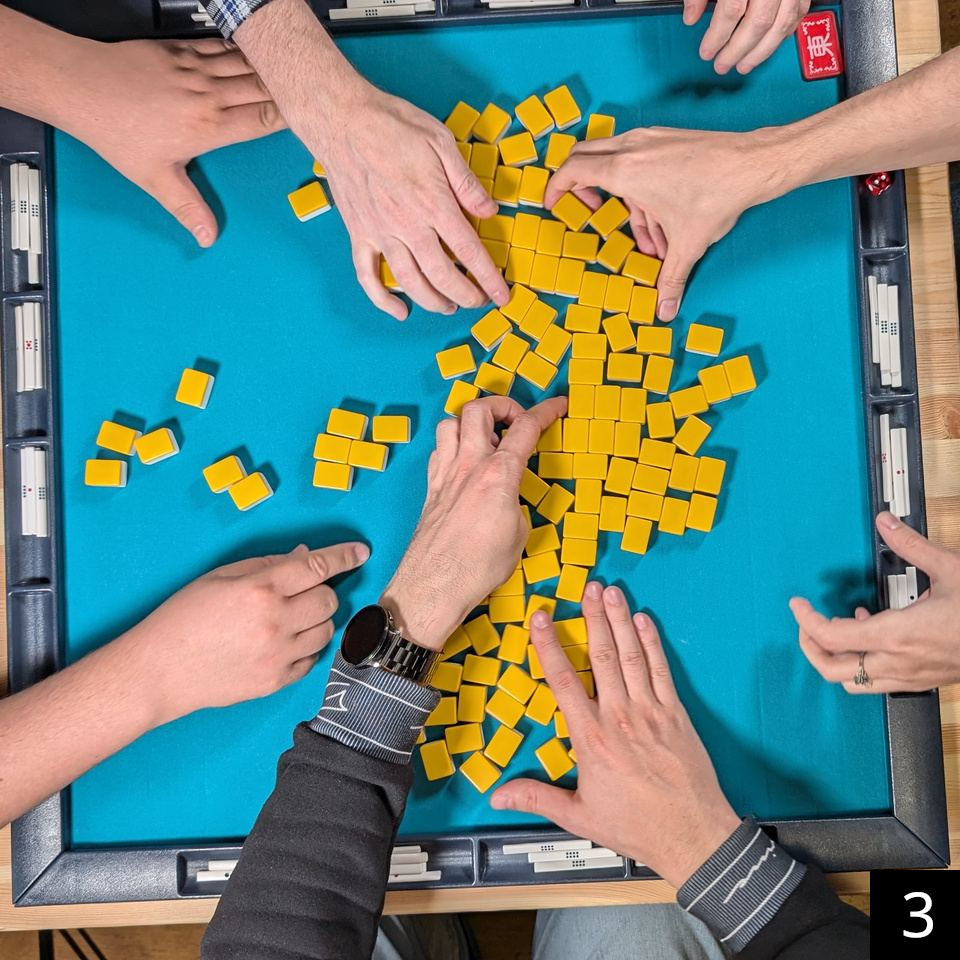
\includegraphics[width=8cm]{03_shuffle.jpg}
	\caption{Порядок перемешивания стены в три этапа}
\end{figure}

Не допускается разрушать и повторно замешивать кусок стены, который уже начал собирать другой игрок. Подобное действие считается дурным тоном и может привести к указанию так не делать.

Некоторые игроки при постройке стены ставят дальний ряд на ближний и делают это у борта. Некоторые техники жульничества основаны на том, что проще закладывать себе тайлы для подмены на верхний ряд, поэтому лучше будет отодвинуть оба ряда от борта и поставить ближний ряд сверху дальнего. Однако и это не лучший способ --- в процессе отодвигания стена может порушиться и придется перемешивать тайлы и набирать заново. Поэтому наиболее быстрый и надежный способ построения стены следующий: набираем два ряда по 17 у борта, равняем их, аккуратно отодвигаем дальний ряд туда, где будет стоять стена, отодвигаем ближний ряд от борта, после чего ставим его поверх дальнего ряда. 

\begin{figure}[H]
	\centering
	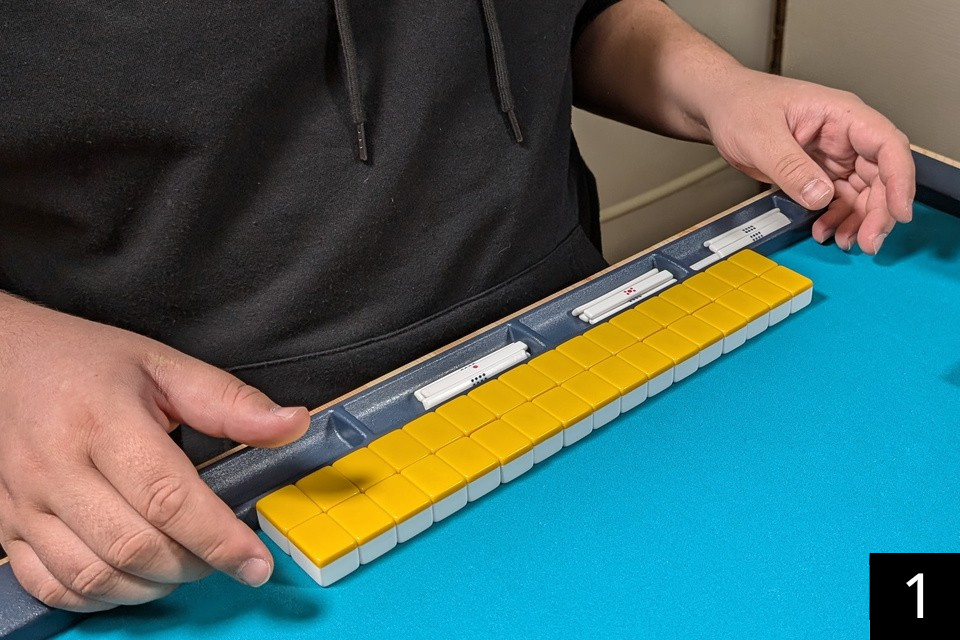
\includegraphics[width=8cm]{04_wall.jpg}
	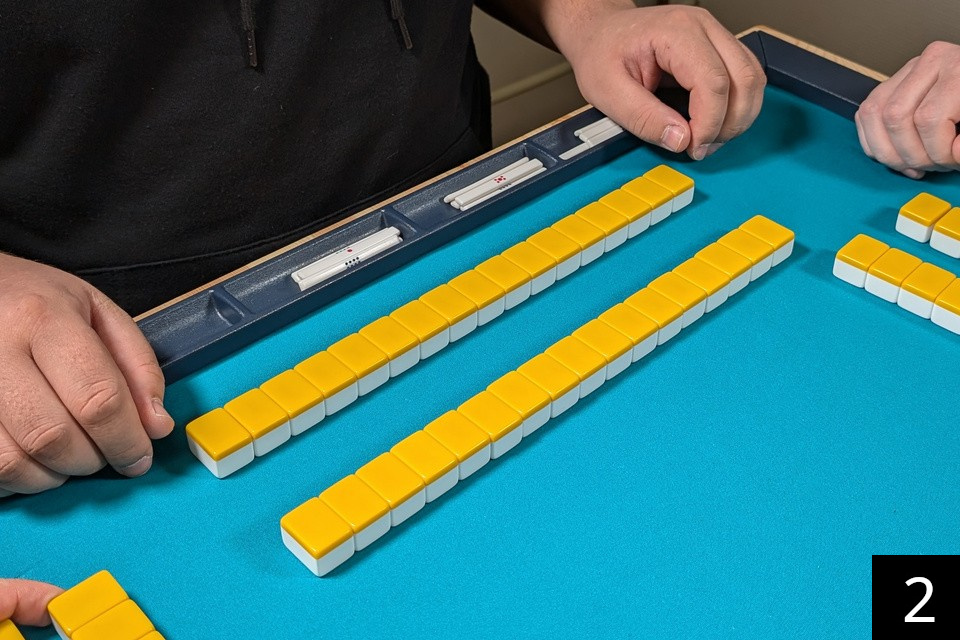
\includegraphics[width=8cm]{05_wall.jpg}
	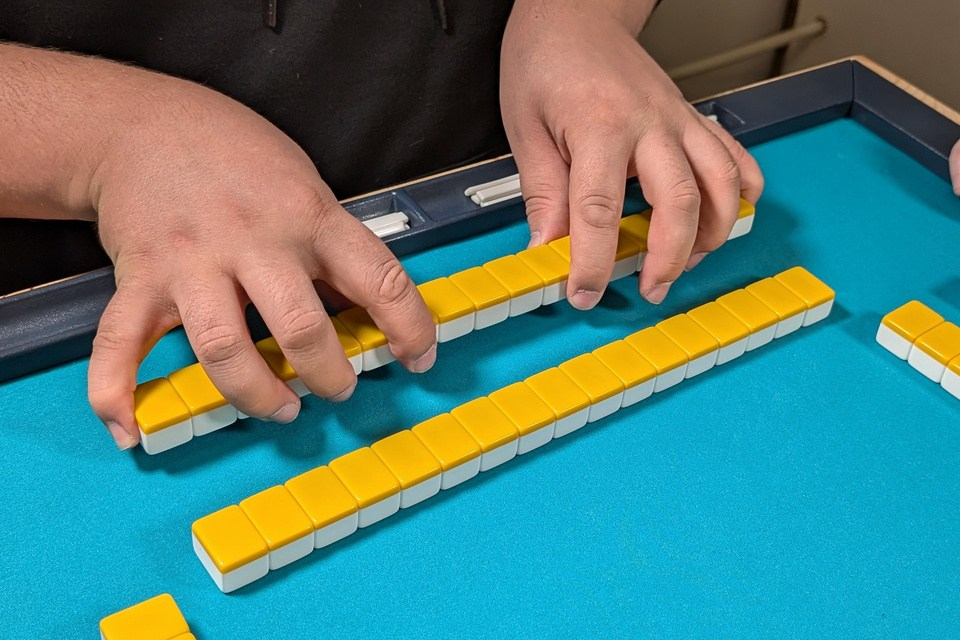
\includegraphics[width=8cm]{06_wall.jpg}
	\caption{Порядок построения стены}
\end{figure}

При подъеме ряда стены поверх другого ряда игрок может случайно разрушить поднимаемый ряд. 

\begin{figure}[H]
	\centering
	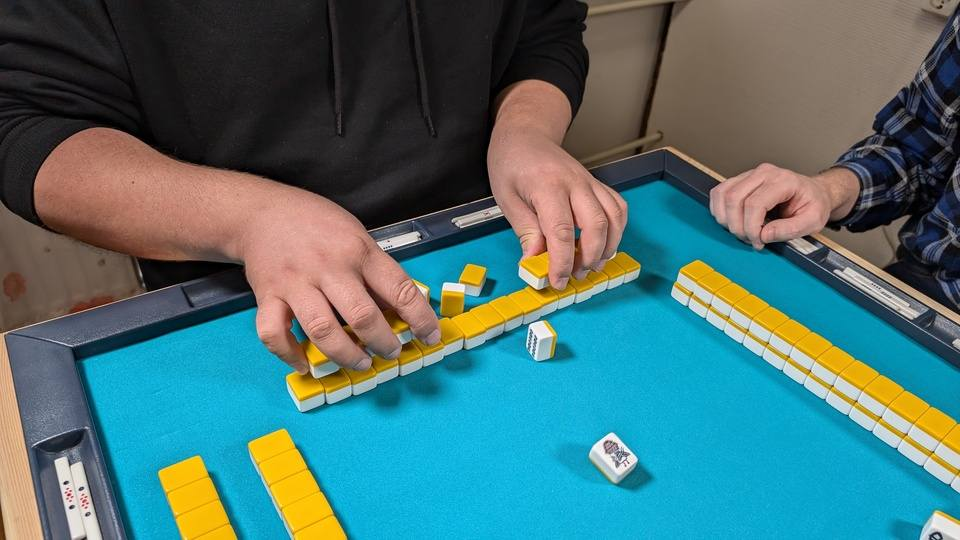
\includegraphics[width=8cm]{07_wall.jpg}
	\caption{Ошибка при установке верхнего ряда}
\end{figure}

\newpage

В случае, если тайлы скользкие или игрок не уверен в том, сможет ли он поднять ряд стены, рекомендуется поднимать ряд стены по частям.

\begin{figure}[H]
	\centering
	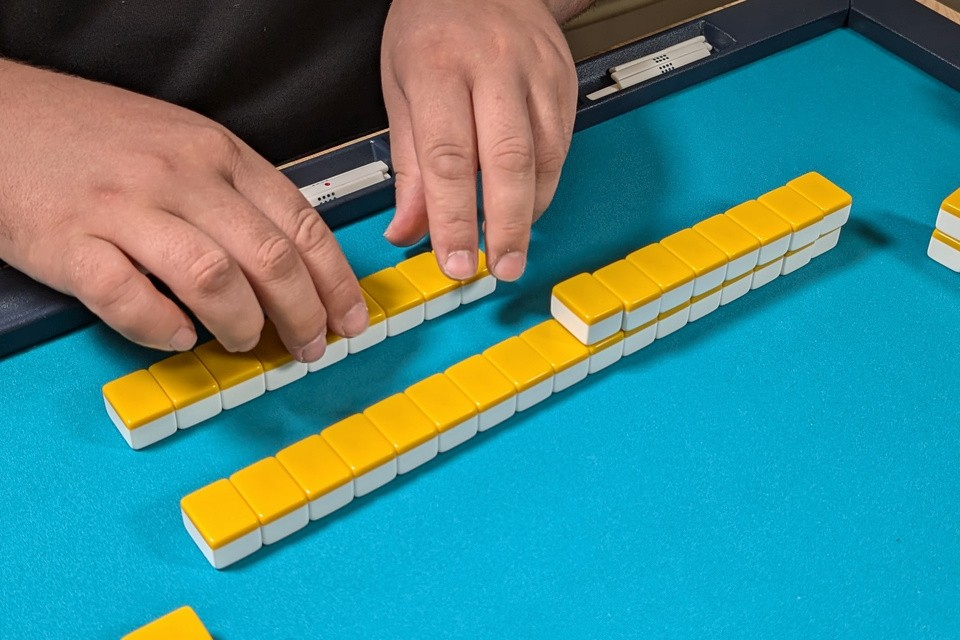
\includegraphics[width=8cm]{08_wall.jpg}
	\caption{Подъем ряда стены по частям}
\end{figure}

Отодвигать ряд стены следует движениями влево-вправо, чтобы исключить возможность разрушения построенного ряда.

\begin{figure}[H]
	\centering
	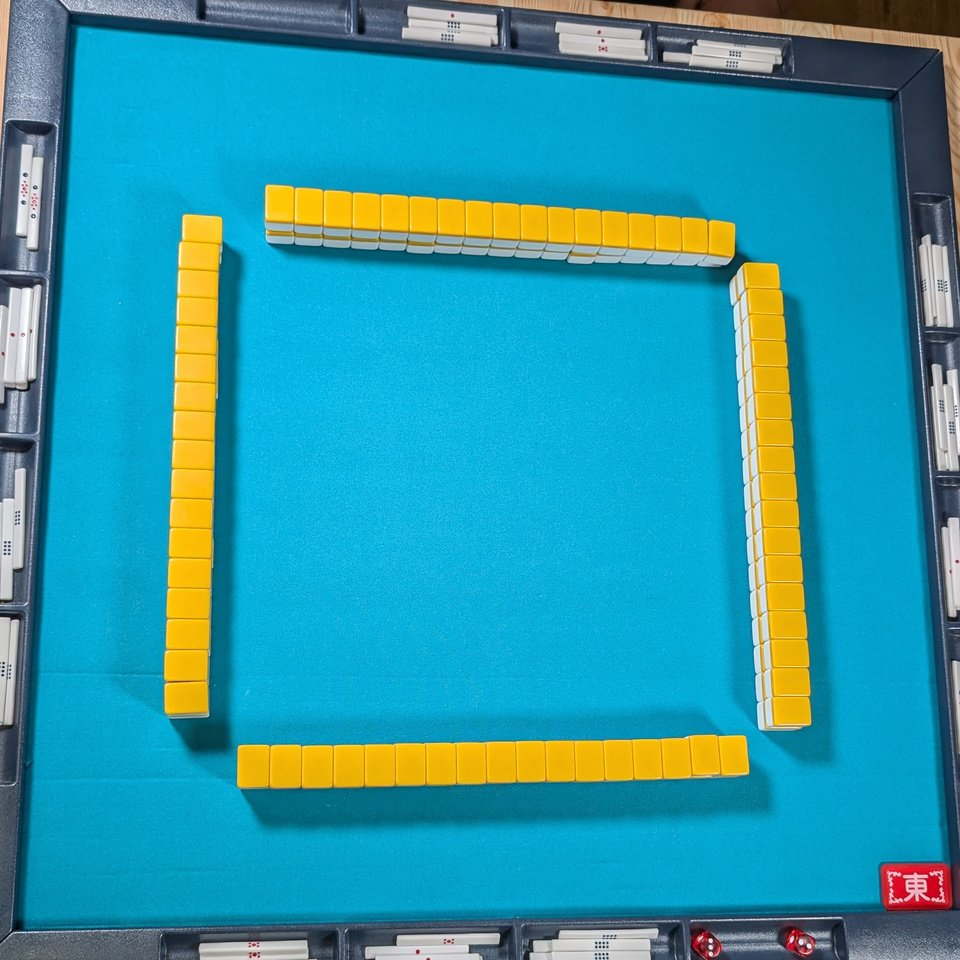
\includegraphics[width=8cm]{09_wall.jpg}
	\caption{Изначальное расположение стены}
\end{figure}

\newpage

После построения стены рекомендуется слегка повернуть ее так, чтобы правый ряд был чуть выдвинут вперед:

\begin{figure}[H]
	\centering
	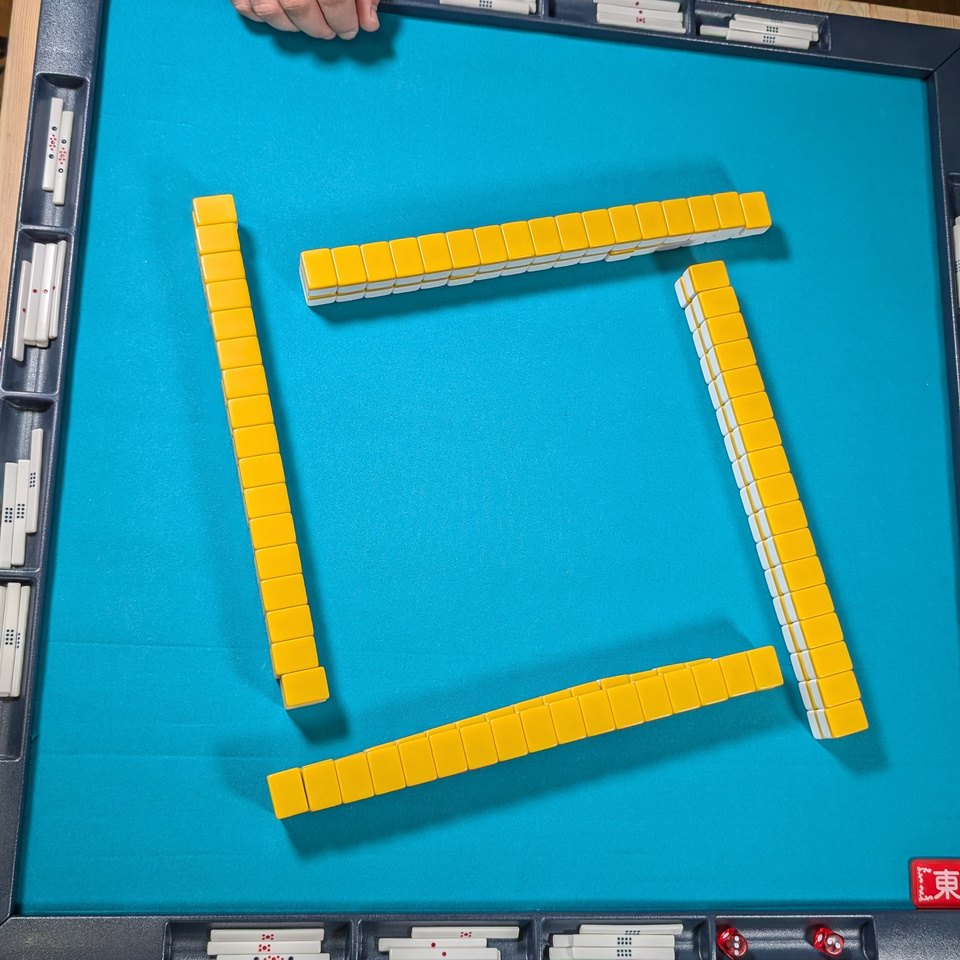
\includegraphics[width=8cm]{10_wall.jpg}
	\caption{Расположение стены}
\end{figure}

Это нужно, во-первых, чтобы тоймену было чуть проще тянуться за тайлом (а чтобы по мере разбора ему тянуться не стало сложнее, рекомендуется пододвигать свою стену время от времени), во-вторых, чтобы игроку слева было видно, есть ли в нижнем ряду тайл --- когда стена стоит параллельно его взгляду, увидеть тайл может быть сложно, в-третьих, некоторые тайлы могут быть великоваты для конкретного стола и поворотом стен игроки получают дополнительное пространство для размещения своих рук перед собой. Двигать стену рекомендуется до броска кубиков, т.к. формально бросок кубиков является началом раздачи, и случайное разрушение стены после него может наказываться штрафом. Если места хватает для всех рук и дискардов, поворачивать стены не требуется.

Перемешивание тайлов, построение стены и сортировка тайлов в своей руке (как при наборе тайлов так и во время игры) --- это действия, которые можно и нужно делать двумя руками, однако дальнейшие действия следует выполнять \textbf{одной рукой} (желательно доминантной). В случае, если игрок использует обе руки для взятий, объявлений и сбросов, судья может вынести вежливое указание играть единственной рукой. Мотивация данного ограничения исходит из того, что при игре двумя руками возрастает вероятность некорректных или даже намеренно обструктивных действий, поэтому такой практики следует избегать.

\newpage

В некоторых источниках рекомендуют также делать разлом стены "лесенкой" 6-5-6, однако в других источниках, напротив, рекомендуют от этой практики отказаться:

\begin{figure}[H]
	\centering
	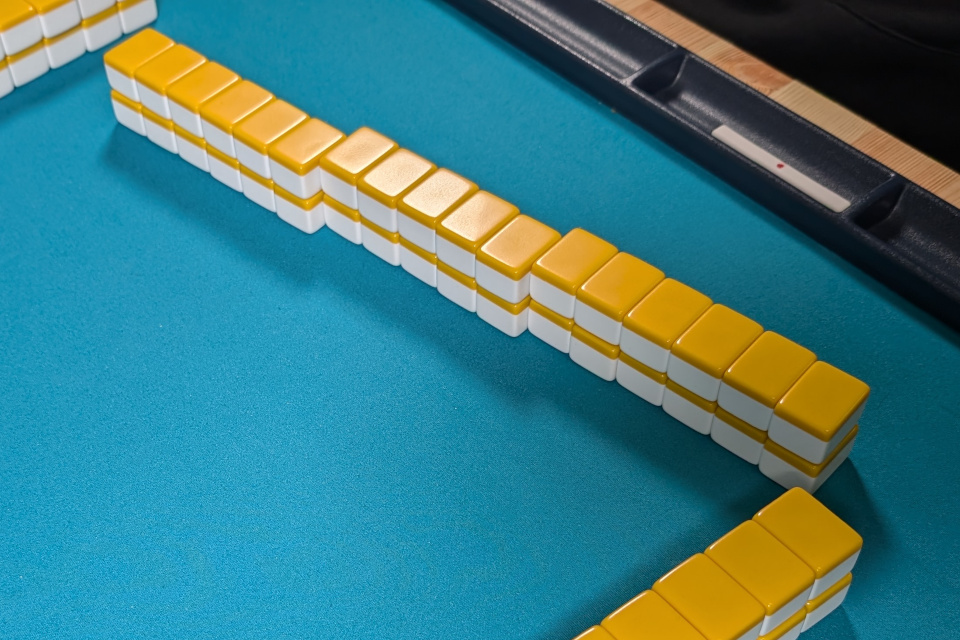
\includegraphics[width=8cm]{11_wall.jpg}
	\caption{Стена лесенкой}
\end{figure}

Считается, что такой разлом позволяет дилеру проще понять, где нужно сделать разлом, но это может не сработать, если самому сделать сдвиги неправильно. Другие аргументы за сдвиг:
\begin{itemize}
	\item Если сдвинутой стене случайно толкнуть верхний ряд --- не упадет верхний тайл на другом конце стены.
	\item Сдвиг делают, чтобы показать, что не собираются жульничать (манипуляции с такой стеной крайне затруднительны и  более очевидны).
\end{itemize} 
В итоге однозначных доводов против лесенки нет, однако требовать этого от всех игроков затруднительно, так что решение о сдвиге остается за игроком.

\subsubsection{Бросок кубиков, разлом, мертвая стена}

После броска кубиков дилеру рекомендуется вслух проговорить выброшенное число, убедиться, что все игроки увидели то же самое (бывают случаи когда кому-то показалось другое число), и сразу же забрать и отложить кубики в правый угол стола. Обратите внимание, что именно кубики обозначают текущего дилера в раздаче. Индикатор раунда является индикатором первого дилера, он должен лежать у игрока, который являлся первым дилером в игре, и не должен перемещаться во время игры (только переворачиваться в начале южного раунда).

Индикатор первого дилера и кубики должны располагаться либо в зоне сетов справа от руки, либо в лотке для очков. Не следует класть кубики или индикатор слева от руки, поскольку там располагается зона сетов другого игрока.

Разлом стены может выполнить игрок, на чью стену указал бросок кубиков, также разлом может выполнить дилер одновременно со своим первым взятием. Обратите внимание, что поскольку стена всегда содержит 17 тайлов, то, когда на кубиках выброшено больше 8 --- проще отсчитать остаток с левой части стены --- например 7, когда выброшено 10, или 5, когда выброшено 12.

\newpage

Игрок, в чьей стене находится изначальный индикатор доры, должен перевернуть ее, не замедляя процесса набора тайлов (если до него дошла очередь взять тайлы, то следует сначала взять их, а потом, пока тайлы берут другие игроки, открыть индикатор). Следует воздержаться от переворачивания индикатора одним пальцем, чтобы случайно не разрушить мертвую стену:

\begin{figure}[H]
	\centering
	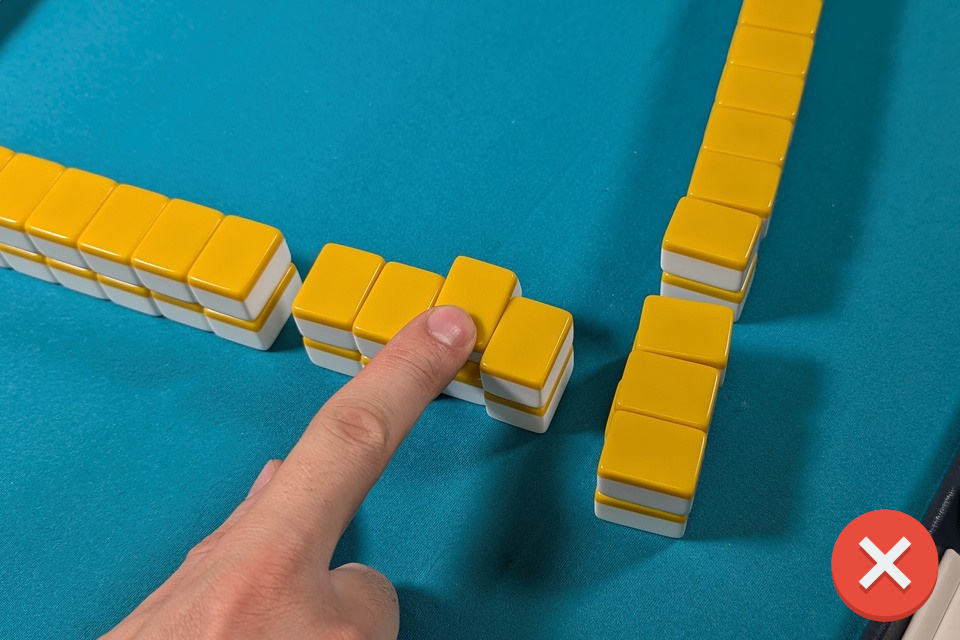
\includegraphics[width=8cm]{12_wall-break.jpg}
	\caption{Не переворачивайте индикатор одним пальцем}
\end{figure}

Снятие первого тайла замены в мертвой стене --- действие не обязательное, но рекомендуемое:

\begin{figure}[H]
	\centering
	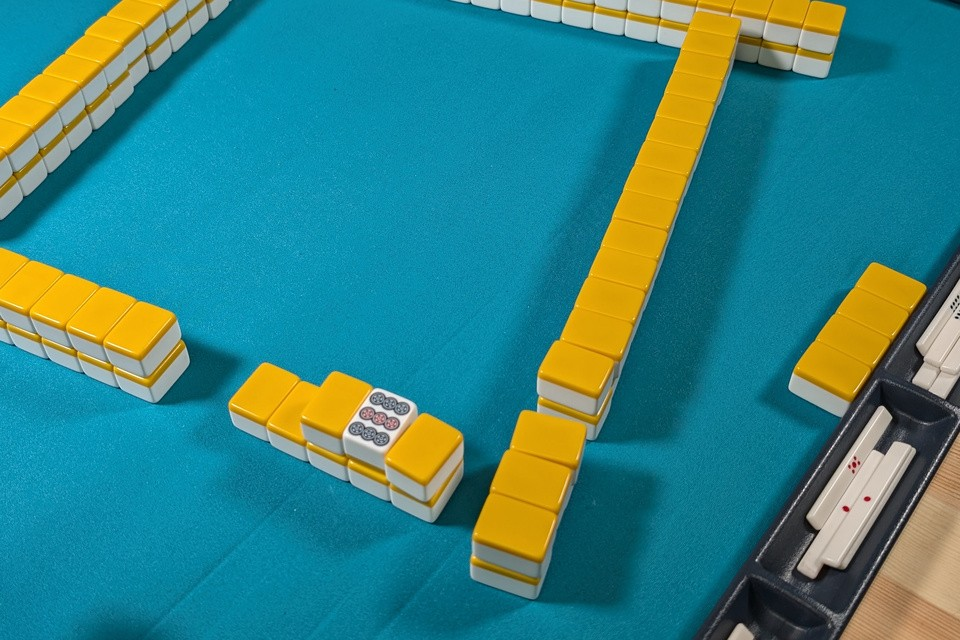
\includegraphics[width=8cm]{13_wall-break.jpg}
	\caption{Мертвая стена со снятым первым тайлом замены}
\end{figure}

Снятый тайл замены может остановить случайное взятие тайла не с того конца стены, т.к. мертвая стена будет визуально отличаться от живой, намекая что брать тайлы из нее не следует. 

Также рекомендуется отделить мертвую стену от живой, сделав небольшой разлом, но опять же, не замедляя процесс набора тайлов. Данное требование не является обязательным, поскольку до третьего ряда дискарда нет особого смысла беспокоиться о том, где кончается живая стена, кроме того, в случае объявления кана исходный разлом может стать неактуальным. В случае, если игрока просят отделить мертвую стену заранее, игроку следует прислушаться к просьбе.

Не следует никаким образом трогать чужие стены --- если нужно каким-либо образом подвинуть часть или всю стену, следует попросить об этом игрока, с чьей стороны находится стена. В целом, рекомендуется прикасаться к любым стенам (за исключением собственных взятий со стены) \textbf{как можно меньше}.

Недопустимо передвигать тайлы из одной стены в другую с целью полностью отделить мертвую стену --- это бессмысленная трата времени, которая к тому же иногда приводит к тому, что у игрока в стене оказывается слишком много тайлов (и такую стену банально неудобно двигать). За попытку передвигать тайлы из чужой стены в свою и наоборот может последовать вежливое указание так не делать.

\begin{figure}[H]
	\centering
	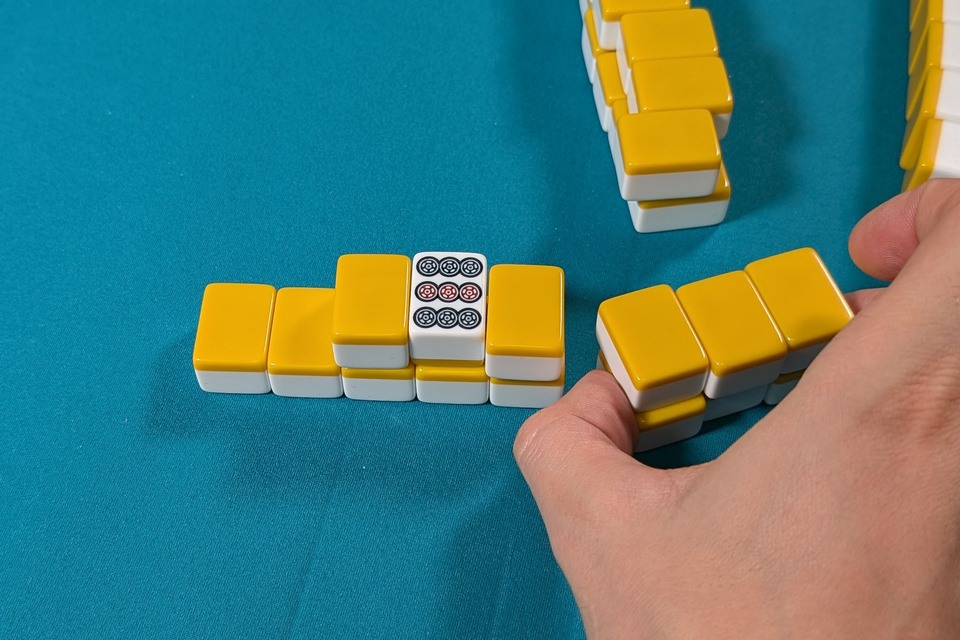
\includegraphics[width=8cm]{14_wall-dont.jpg}
	\caption{Не трогайте чужие стены}
\end{figure}

При изначальном наборе тайлов не следует торопиться и брать тайлы не в свою очередь. Набор тайлов не в свою очередь дезориентирует игроков и приводит к гораздо большим потерям времени, чем если бы все игроки набирали тайлы последовательно.

Дилер в конце начального набора тайлов должен взять первый тайл и тайл через один от него. Брать тайлы следует осторожно, чтобы случайно не перевернуть еще не взятые тайлы, за неоднократное переворачивание тайлов из стены последует вежливое указание так не делать.

\begin{figure}[H]
	\centering
	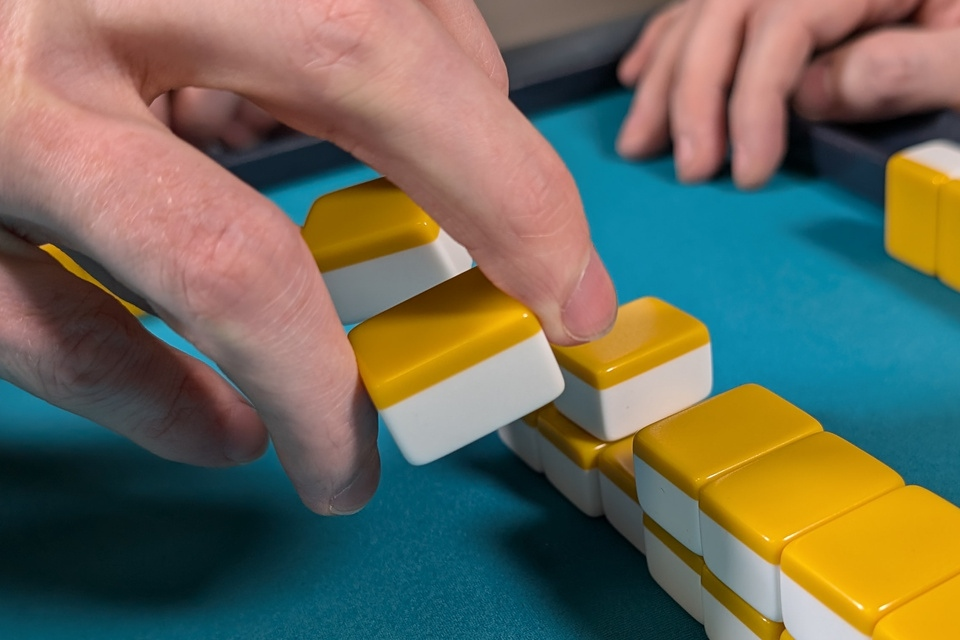
\includegraphics[width=8cm]{15_take-tiles-last-wrong.jpg}
	\caption{\centering Взятие двух тайлов одним движением может \linebreak привести к переворачиванию тайлов в стене}
\end{figure}

\begin{figure}[H]
	\centering
	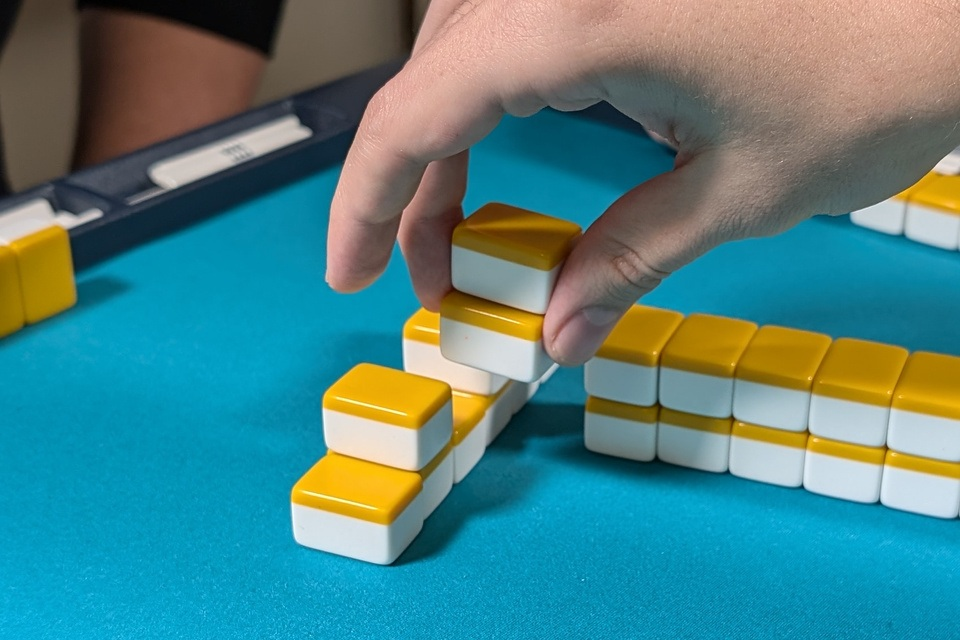
\includegraphics[width=8cm]{16_tiles-get.jpg}
	\caption{Рекомендуется брать последние два тайла по одному}
\end{figure}

Не рекомендуется брать последние тайлы по одному каждым игроком, поскольку это может дезориентировать игроков (например, игрок на западе может по ошибке взять тайлы через один, как это делает дилер). Нарушение порядка разбора может привести к вежливому указанию так не делать.

\subsubsection{Набор тайлов}

Не рекомендуется набирать все тайлы рубашкой вверх и затем открывать всю руку. Это может привести к тому что некоторые тайлы будут вскрыты (в лучшем случае), а ближайшая стена разрушена (в худшем):

\begin{figure}[H]
	\centering
	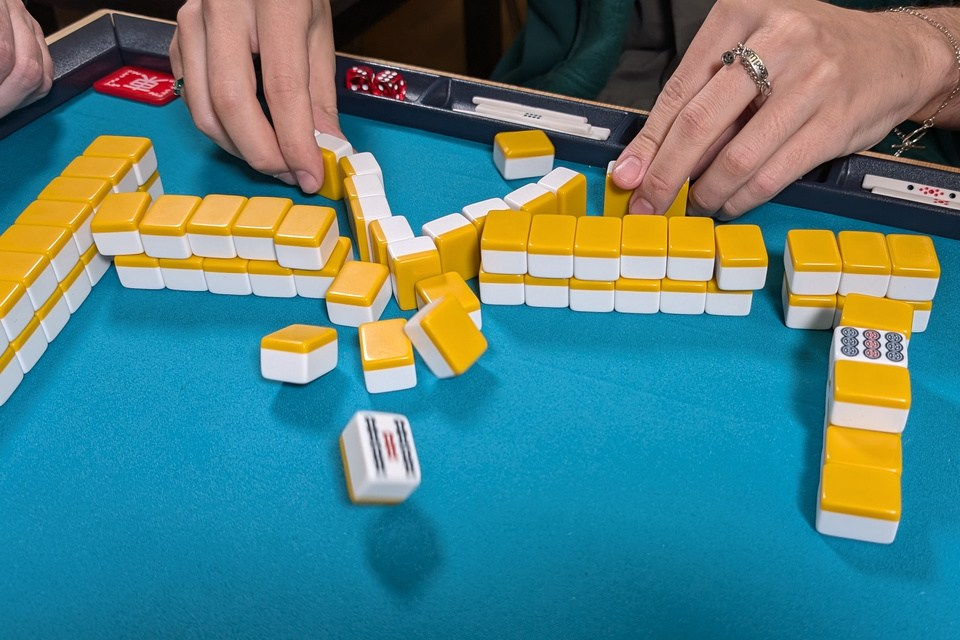
\includegraphics[width=8cm]{17_hand-open.jpg}
	\caption{Типичная ошибка при открытии руки}
\end{figure}

Даже если стол решит не штрафовать игрока и все согласятся на пересдачу тайлов --- это приведет к потере времени. Кроме того, открывая тайлы сразу, игрок может быстрее понять потенциалы своей руки, что сэкономит время на обдумывание первого хода. Если при этом тайлы еще и сортировать, пока другие игроки берут свои, то время экономится еще и на сортировке.

\begin{figure}[H]
	\centering
	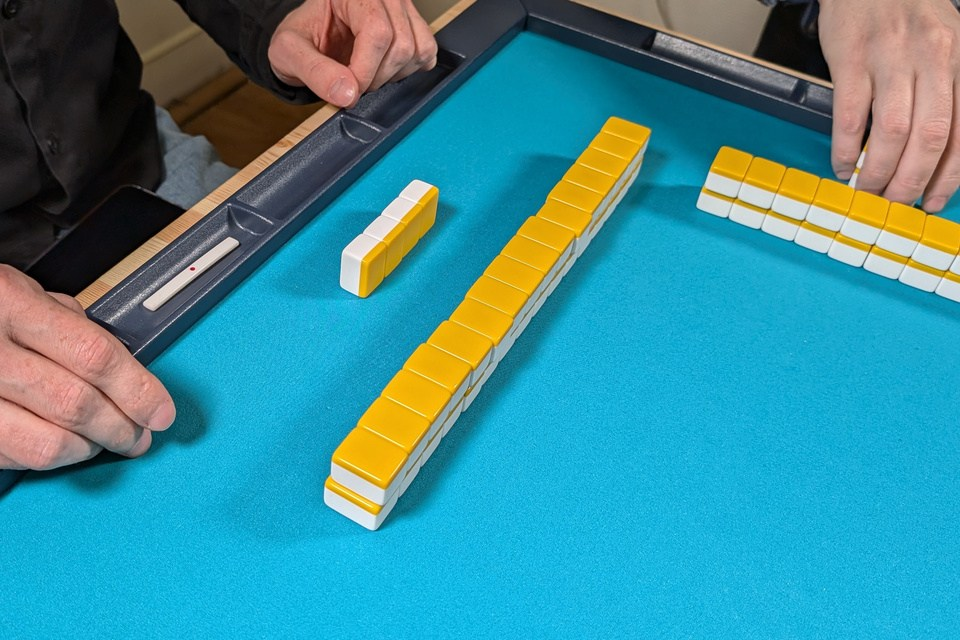
\includegraphics[width=8cm]{18_open-tiles-immediately.jpg}
	\caption{Набор тайлов в руку с одновременным их открытием}
\end{figure}

Отдельно стоит упомянуть, что игроки должны не забывать взять последний тайл, а дилер не должен делать первый ход, пока все игроки не набрали тайлы. Таким образом, именно дилер должен убедиться, что у всех игроков 13 тайлов в начале раздачи, и указать на это игрокам, которые забыли взять последний тайл (чаще всего забывает взять тайл игрок на севере). Нет необходимости пересчитывать тайлы в руках игроков --- достаточно взглянуть на живую стену, в ней должен быть только один свободный тайл в нижнем ряду. Также на последний тайл может обратить внимание игрок на юге, в этом случае игроку на севере следует указать на последний тайл, который не был взят. 

В случае возникновения спорных ситуаций из-за невзятого тайла, разрешить ситуацию следует на первом же круге, в таком случае наказаний не последует, но дилеру и игроку, забывшему взять тайл, будет вынесено вежливое указание быть внимательнее. 

После того как тайлы отсортированы, их следует размещать в один ряд без промежутков. Взятый со стены тайл нужно ставить сбоку от руки на небольшом отдалении. Также допускается класть только что взятый со стены тайл боком на руку (однако это не рекомендуется в случае игры за автостолом, чтобы не допустить случайного переворачивания тайла лицом к оппонентам из-за магнитов внутри тайлов).

\begin{figure}[H]
	\centering
	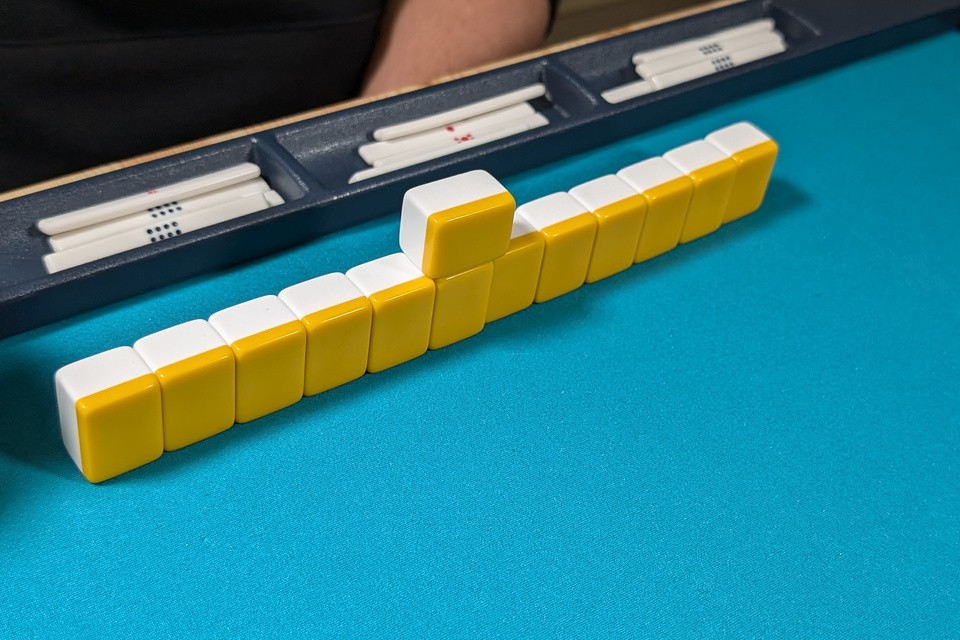
\includegraphics[width=8cm]{62_tsumo-position.jpg}
	\caption{Взятый тайл сверху руки}
\end{figure}

\newpage

Не следует размещать сверху руки более одного тайла.

\begin{figure}[H]
	\centering
	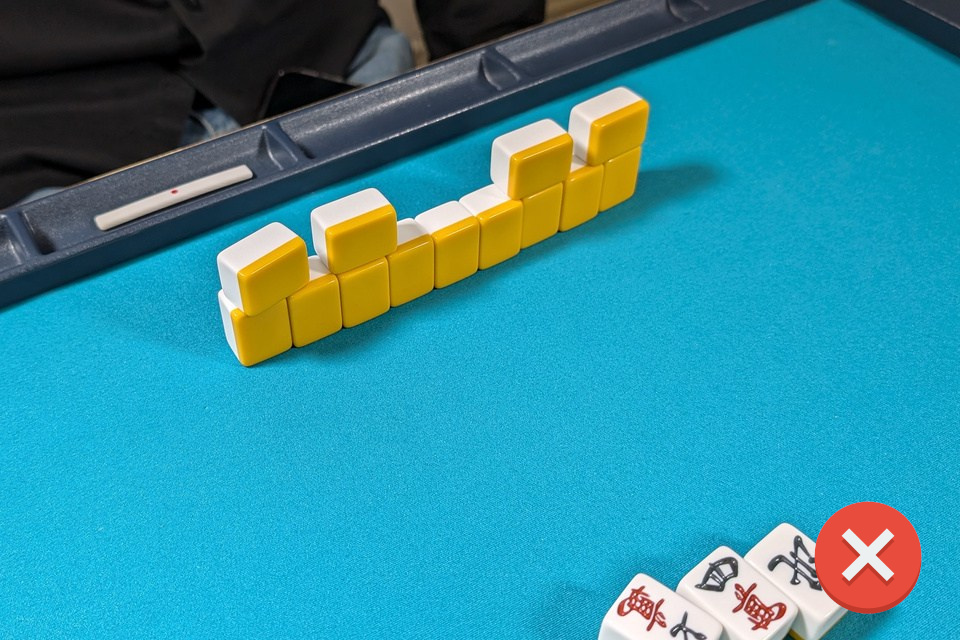
\includegraphics[width=8cm]{63_tiles-position.jpg}
	\caption{Не размещайте тайлы руки сверху}
\end{figure}

\subsection{Процесс игры}

Стол можно условно разделить на несколько зон:
\begin{itemize}
	\item Неиспользуемая зона в центре стола
	\item Зона дискардов и риичи-ставок
	\item Зона стены
	\item Зона рук игроков
	\item Зона сетов игроков
\end{itemize}

\begin{figure}[H]
	\centering
	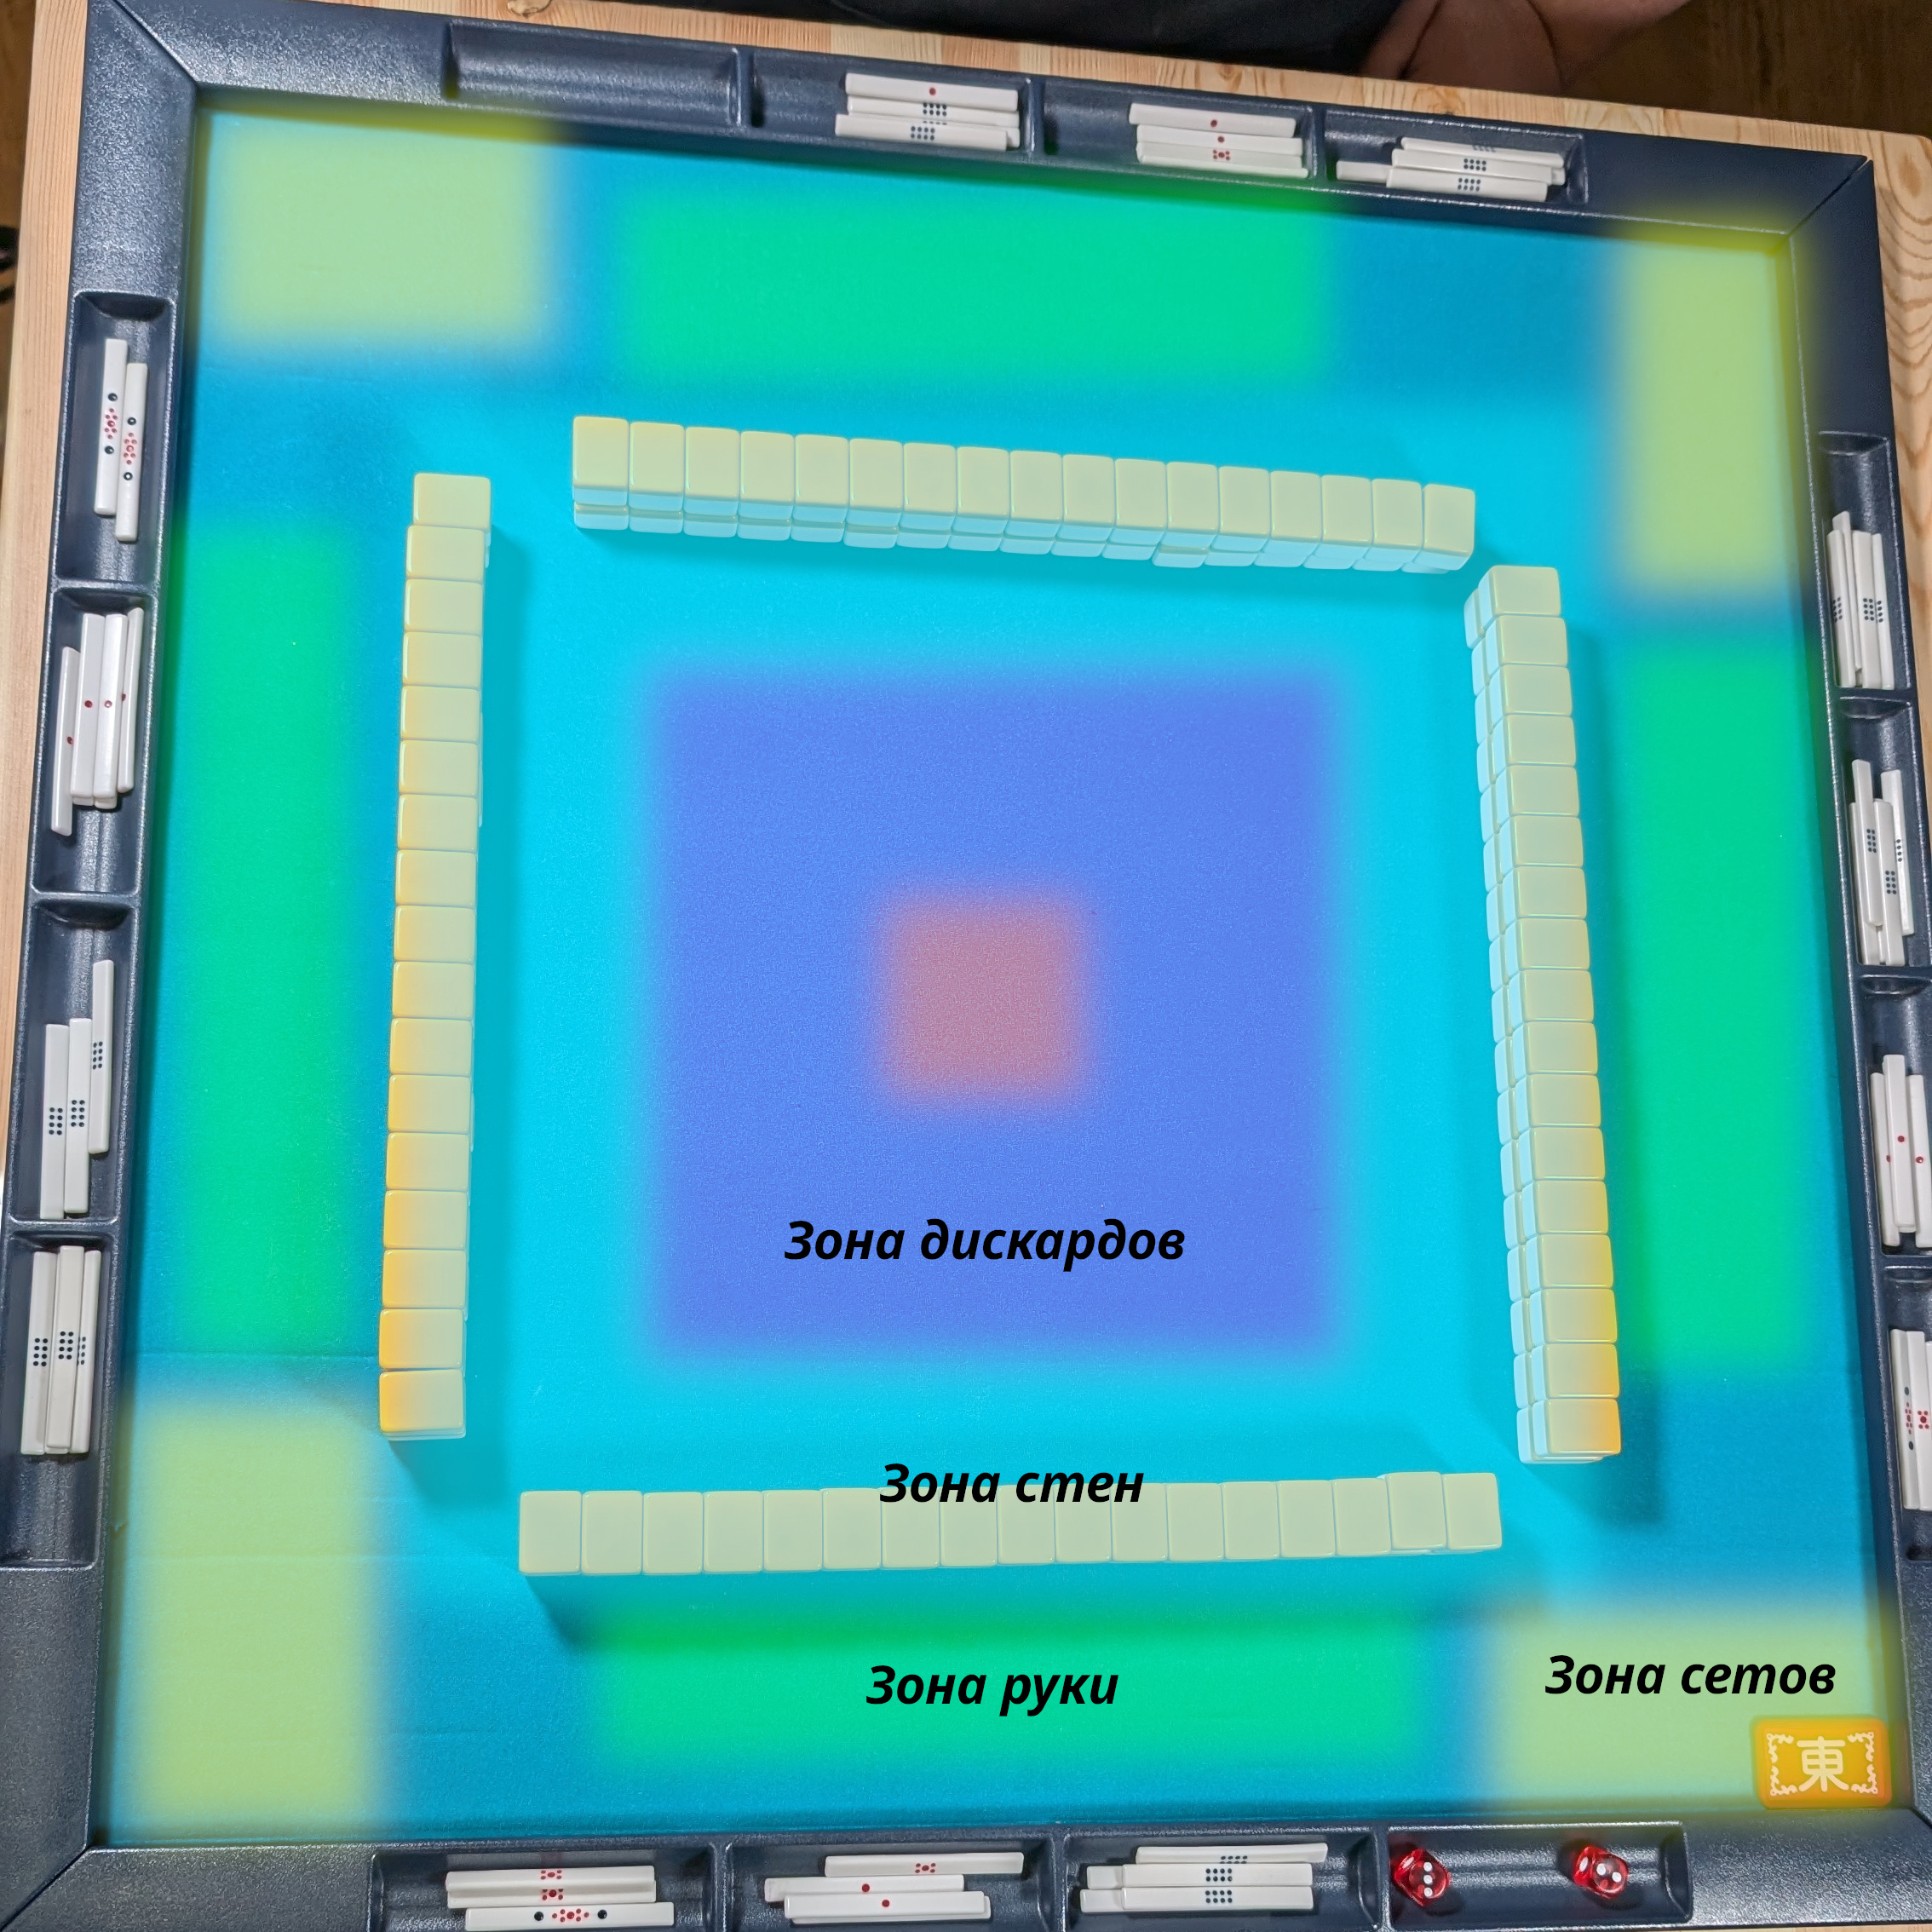
\includegraphics[width=12cm]{zones.jpg}
	\caption{Зонирование игрового стола}
\end{figure}

При выполнении игровых действий игроку следует класть тайлы только в соответствующие зоны. Размещение тайла в неположенном месте может быть воспринято некорректно (например, как победа, хотя вы сбрасываете тайл, или наоборот), и при возникновении спорной ситуации будет воспринято не в пользу игрока, совершившего такое нарушение.

Общая рекомендация для игроков в процессе раздачи --- играть единственной (доминантной) рукой. Не рекомендуется брать тайл со стены одной рукой и сносить другой рукой.

\begin{figure}[H]
	\centering
	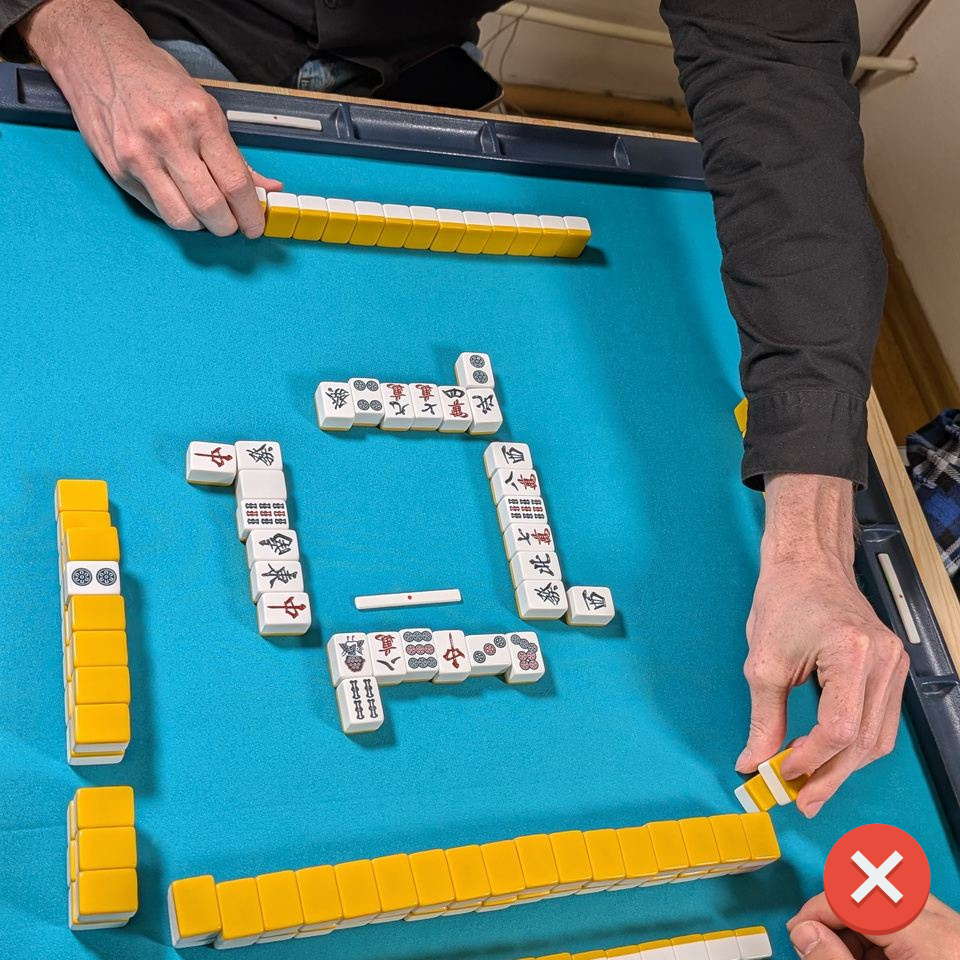
\includegraphics[width=7cm]{64_play-with-one-hand.jpg}
	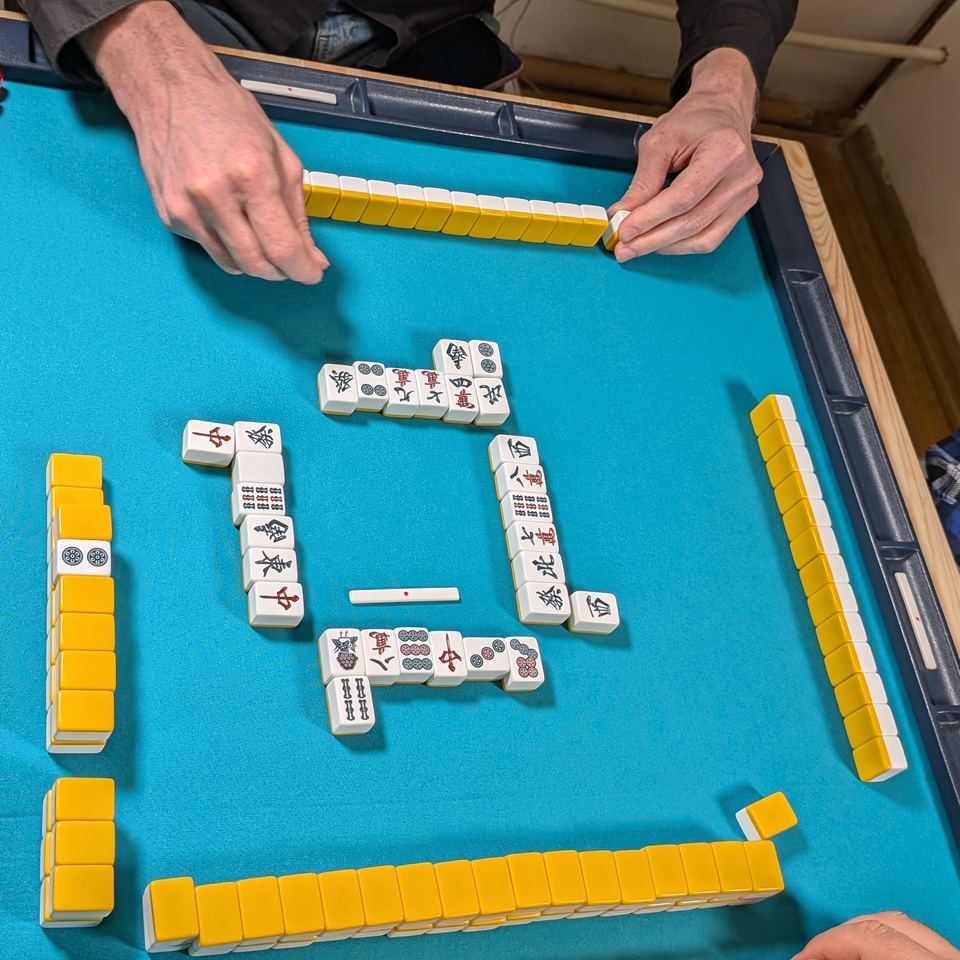
\includegraphics[width=7cm]{65_play-with-one-hand.jpg}
	\caption{Не рекомендуется играть обеими руками}
\end{figure}

\subsubsection{Взятие тайлов из стены}

Рекомендуется следить за тем, чтобы не показывать свои тайлы другим игрокам. Общая рекомендация --- не делать лишних движений. Например, не следует поворачивать тайл лицевой стороной к себе, пока он не окажется в зоне руки, чтобы другой игрок случайно не увидел его:

\begin{figure}[H]
	\centering
	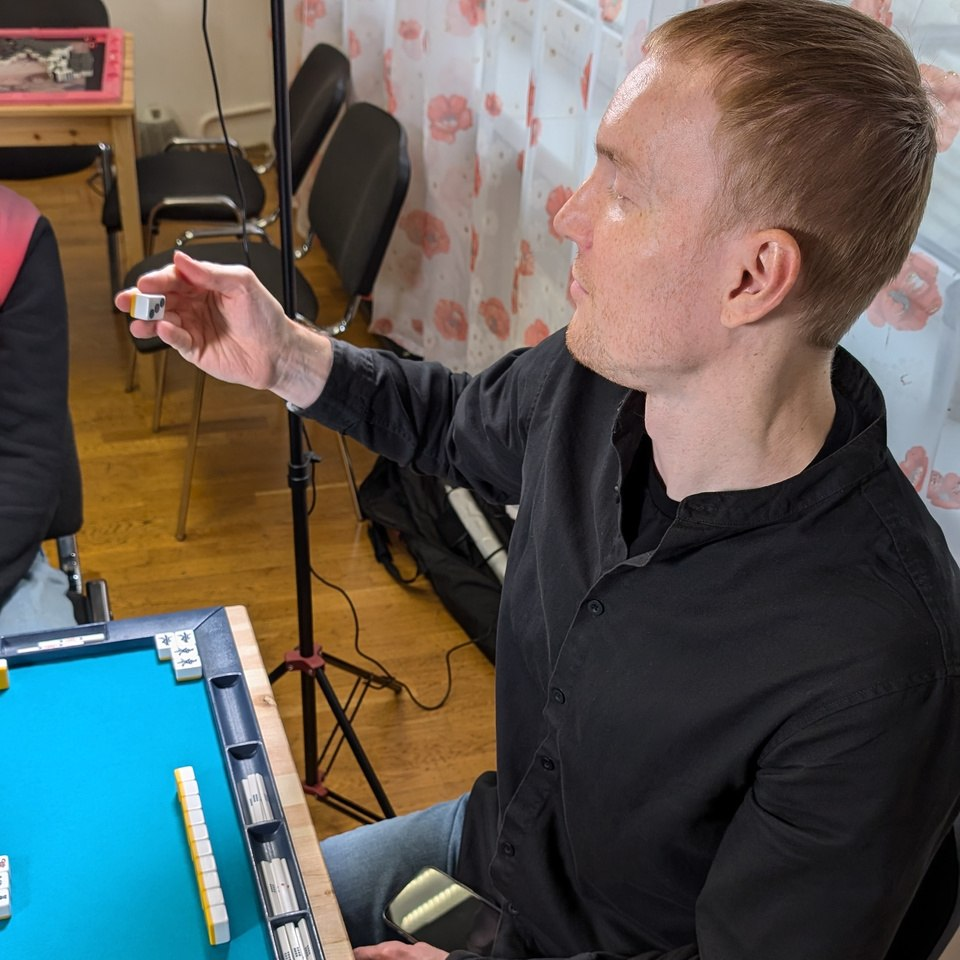
\includegraphics[width=8cm]{19_tile-show.jpg}
	\caption{Не делайте так при взятии}
\end{figure}

Встраивать взятый тайл в руку не рекомендуется до момента сброса, сам же взятый тайл допустимо располагать слева или справа от руки на небольшом отдалении. Допустимо также расположить взятый тайл сверху игровой руки, поставив его на бок, однако следует избегать этого при игре наборами для автостола, поскольку магнит внутри тайла может развернуть тайл лицевой стороной к игрокам. В случае игры на камеру следует позаботиться о том, чтобы зрителям был виден тайл, который только что был взят.

Игрок вправе решать, хочет ли он сделать объявление или взять тайл со стены, только до того момента, пока он не коснулся тайла в стене. Отмена взятия со стены и взятие сета вместо этого не допускается. В случае, если другой игрок делает объявление с последнего дискарда и последовательность ходов изменяется, игрок должен вернуть взятый тайл обратно в стену (для избежания путаницы в этом случае и введена рекомендация не встраивать тайл в руку до момента сброса).

Не спешите со взятием тайлов из стены. Если другие игроки еще не увидели сброс предыдущего игрока, не начинайте тянуться за новым тайлом.

\begin{figure}[H]
	\centering
	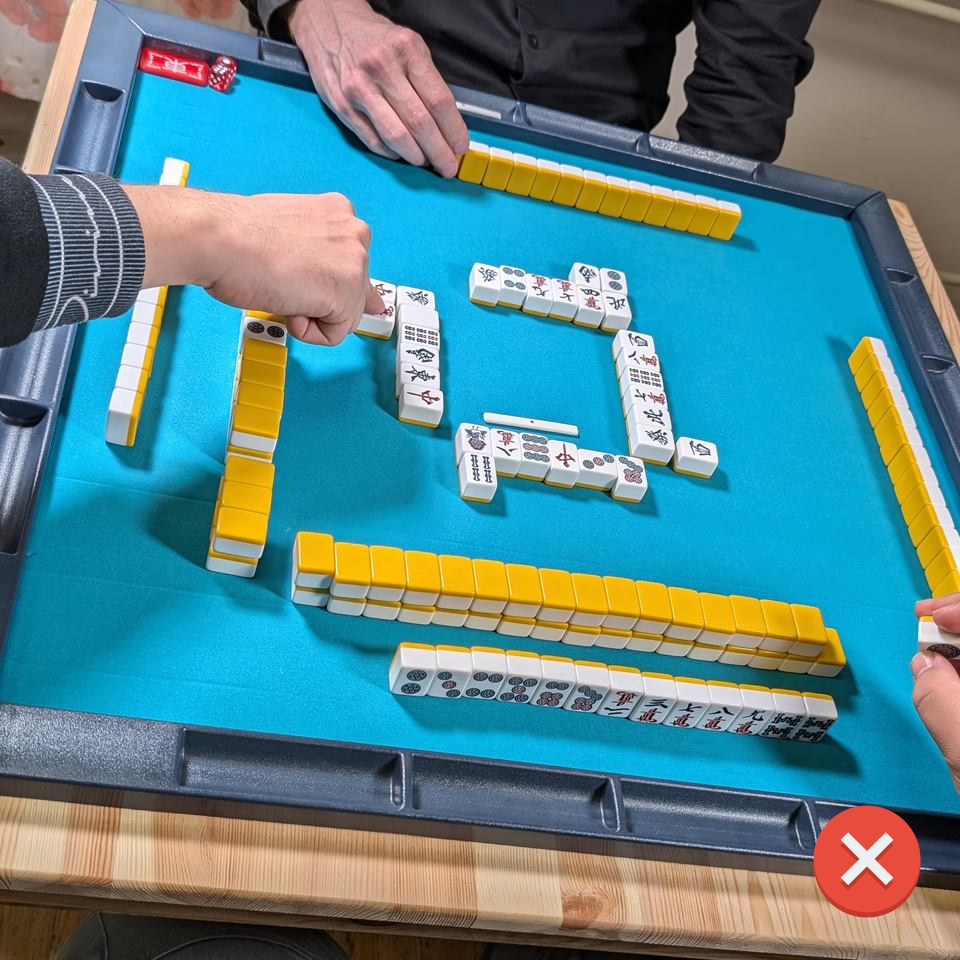
\includegraphics[width=8cm]{68_dont-rush.jpg}
	\caption{Не спешите при взятии тайла со стены}
\end{figure}

\subsubsection{Сброс тайлов}

После первого сброса дилера, игроку на южной стороне рекомендуется убедиться, что все остальные игроки отсортировали руки и готовы продолжать игру, и только после этого делать свое взятие.

Старайтесь выполнять сброс тайла так, чтобы все игроки видели значение тайла одновременно. Некоторые игроки при сбросе тайла перекрывают видимость игроку слева, это приводит к тому, что игрок справа (чей ход следующий) видит тайл раньше игрока слева и делает свое взятие, а игрок слева, увидев тайл позже, решает объявить на нем пон или кан. Задержка приведет к тому, что игрок либо не сделает объявление, подумав что следующий тайл уже взяли (хотя технически он имеет на это право), либо к тому что пон/кан будет объявлен, но игрок справа будет знать каков следующий тайл в стене. Лучше такого избегать, в том числе, игрокам не стоит торопиться брать свой тайл после сброса слишком быстро, стоит убедиться что все игроки за столом точно видели сброс и не делают на нем объявления.

\newpage

Сброс следует делать по шесть тайлов в ряд (следить за тем чтобы начинать второй ряд не раньше --- после пятого тайла, и не позже --- после седьмого). Первый сброшенный тайл в новом ряду допускается разместить не у левого края, но при последующих сбросах его следует выровнять:

\begin{figure}[H]
	\centering
	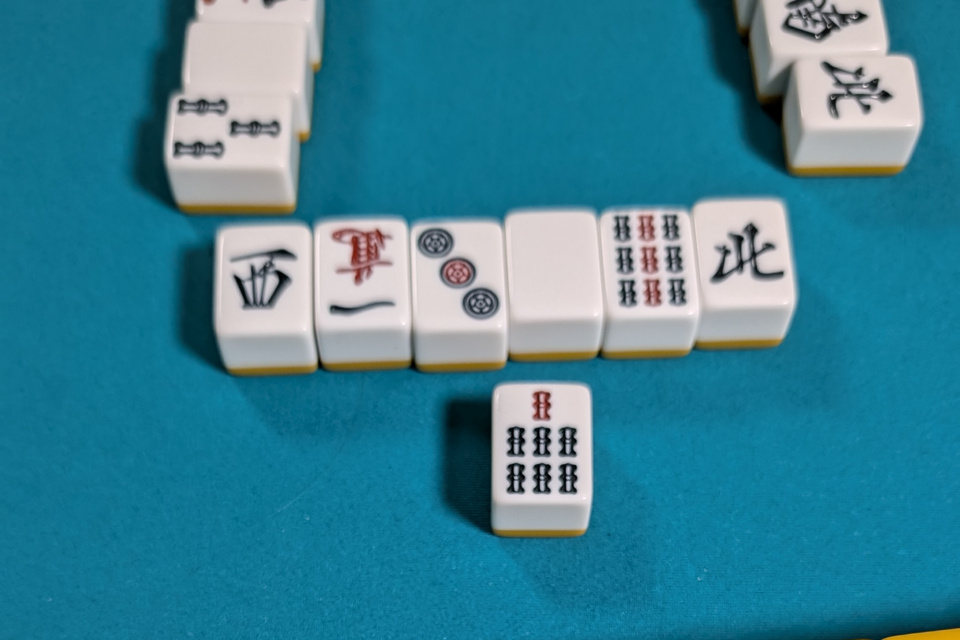
\includegraphics[width=8cm]{20_last-discard-one-tile.jpg}
	\caption{Расположение дискарда}
\end{figure}

В случае, если в третьем ряду уже лежит 6 тайлов, а тайлы в стене еще остались, следует продолжить третий ряд, а не начинать четвертый.

Сбрасываемый тайл следует класть сразу в зону дискарда. Не допускается открывать сбрасываемый тайл рядом с рукой (поскольку это могут воспринять как объявление победы).

\begin{figure}[H]
	\centering
	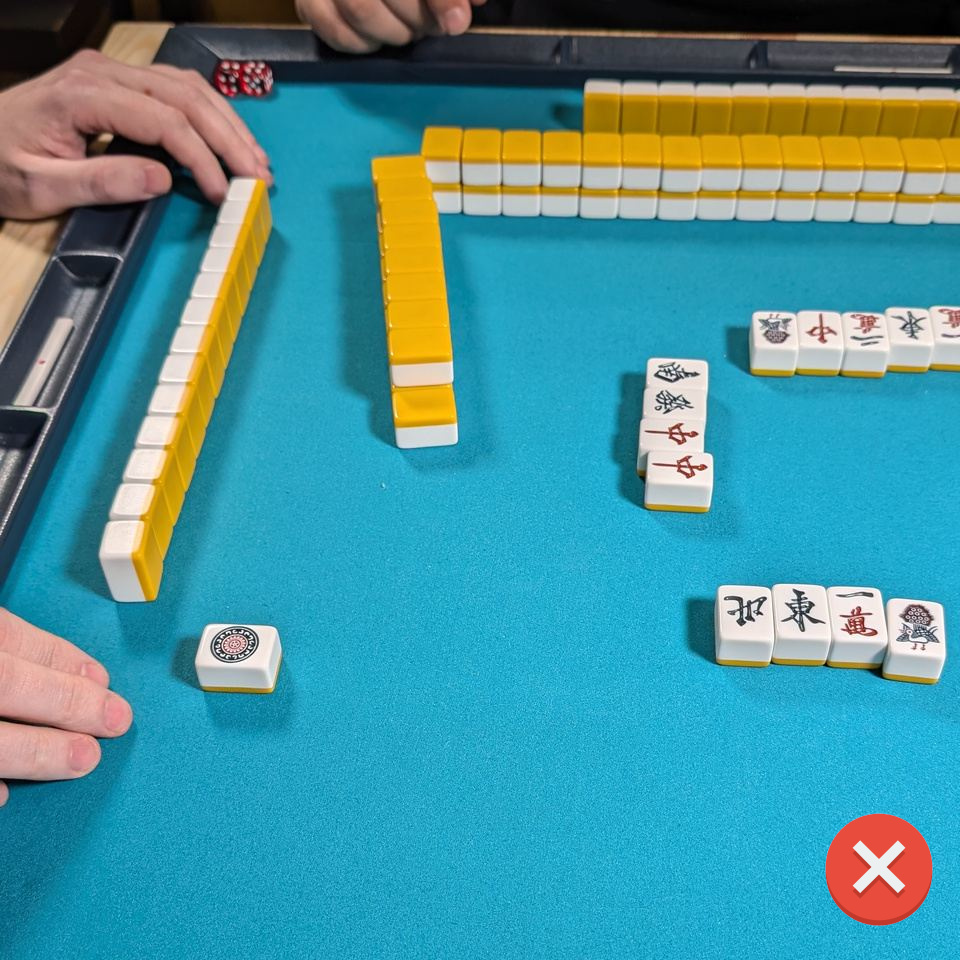
\includegraphics[width=8cm]{70_discard-to-proper-place.jpg}
	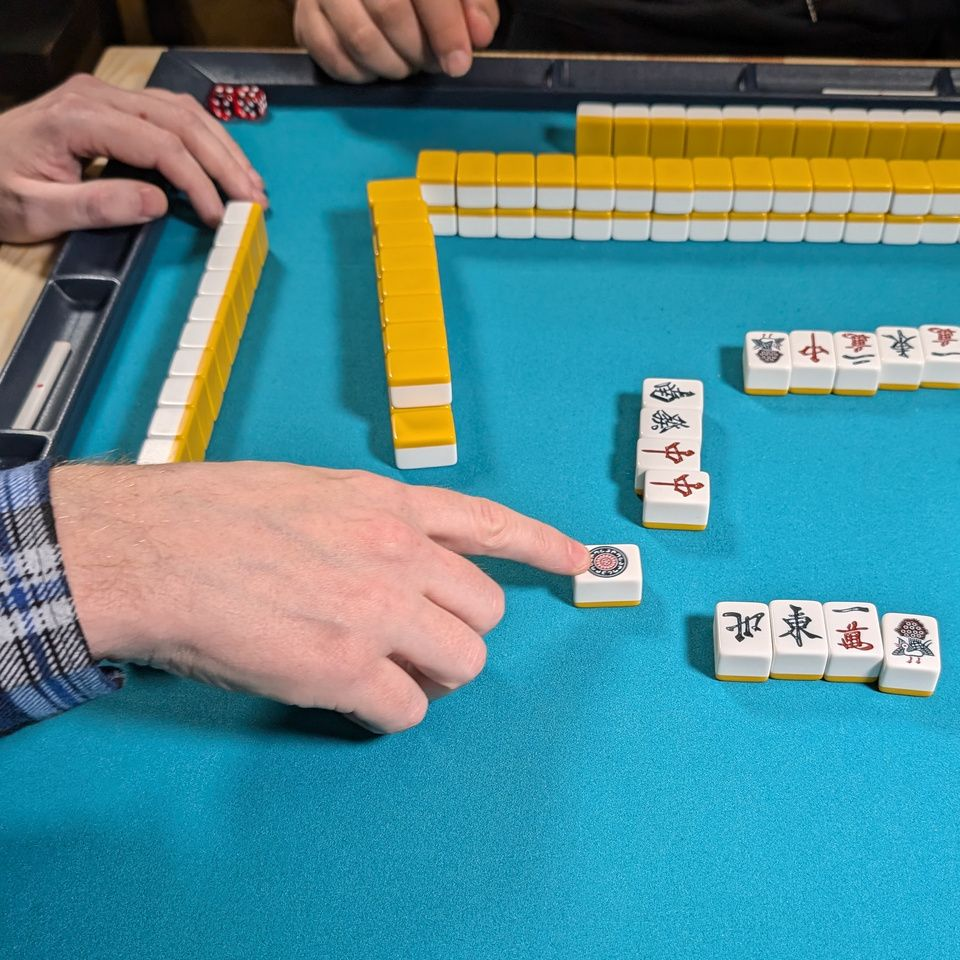
\includegraphics[width=8cm]{71_discard-to-proper-place.jpg}
	\caption{Не делайте так при сбросе}
\end{figure}

\newpage

Следите за упорядоченностью своего дискарда. Хаос в дискарде является дурным тоном и может вызвать спорные ситуации (например, с выявлением принадлежности тайла дискарду того или иного игрока):

\begin{figure}[H]
	\centering
	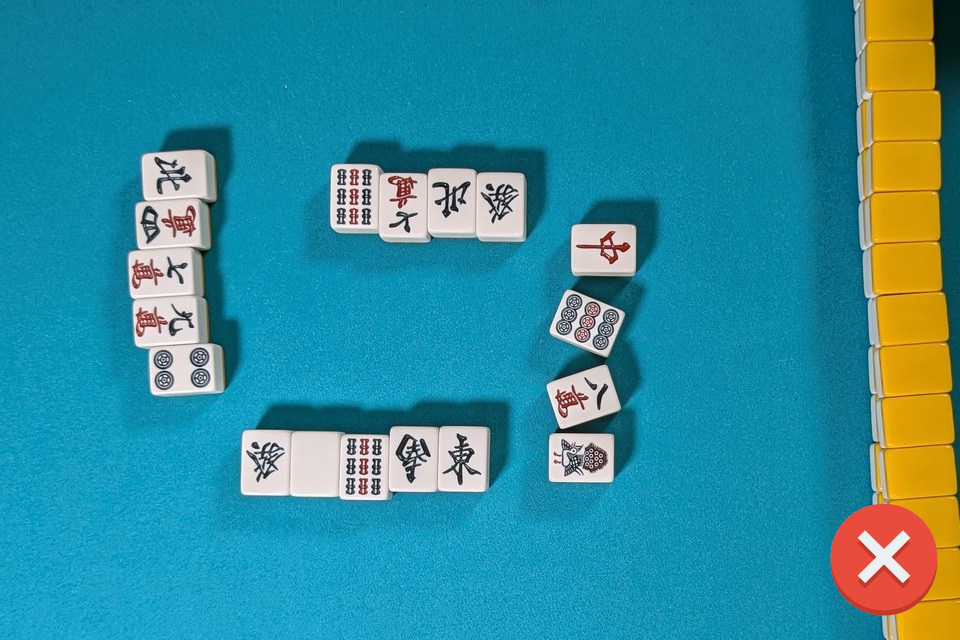
\includegraphics[width=8cm]{21_chaotic-discard.jpg}
	\caption{Хаос в дискарде у игрока справа}
\end{figure}

Допускается поправить или переместить свой дискард в процессе игры, чтобы не допустить перемешивания дискардов или для упорядочивания своего дискарда. Рекомендуется делать это двумя пальцами как показано на рисунке. Не закрывайте дискард руками при перемещении, чтобы вас не заподозрили в нечестной игре.

\begin{figure}[H]
	\centering
	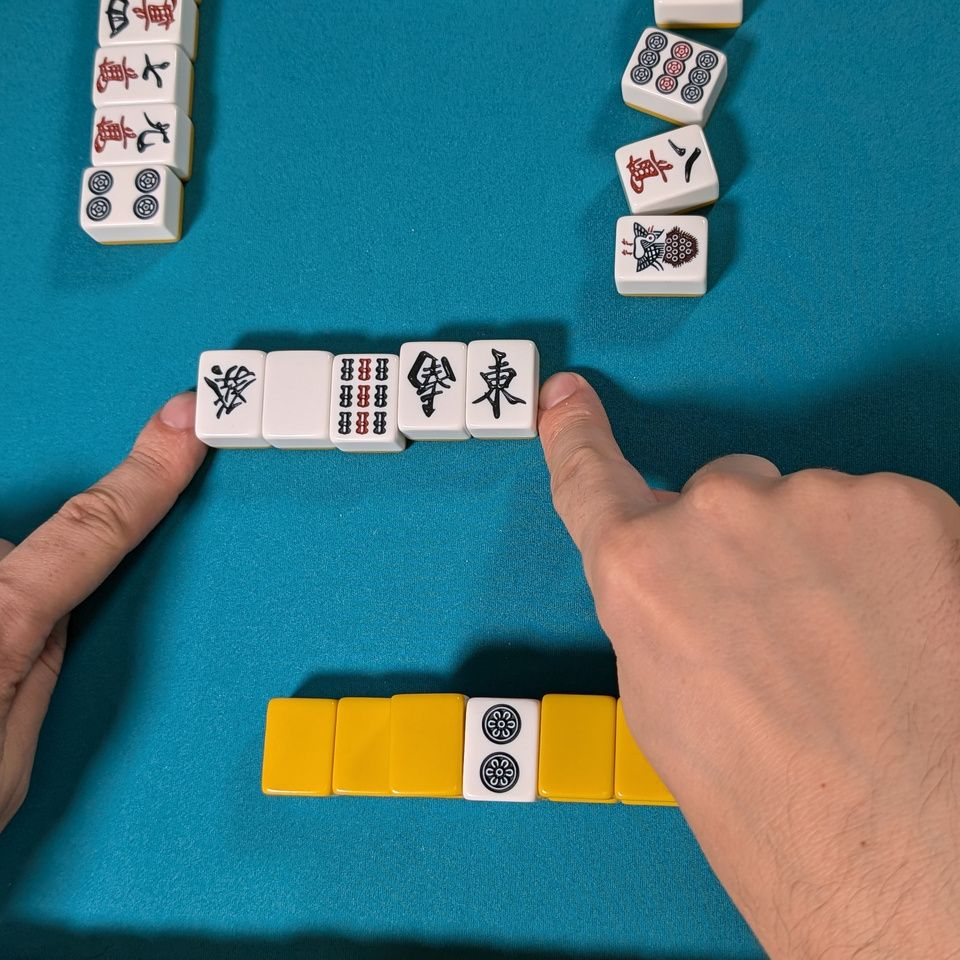
\includegraphics[width=8cm]{67_move-discard.jpg}
	\caption{Корректное перемещение дискарда или его части}
\end{figure}

\newpage

Не играйте с собственным дискардом. Некоторые игроки любят перевернуть симметричную часть дискарда, или заменить тайл в верхнем ряду дискарда таким же сбрасываемым тайлом. Любые подобные действия являются дурным тоном и дают повод усомниться в честной игре, поэтому их следует избегать.

\begin{figure}[H]
	\centering
	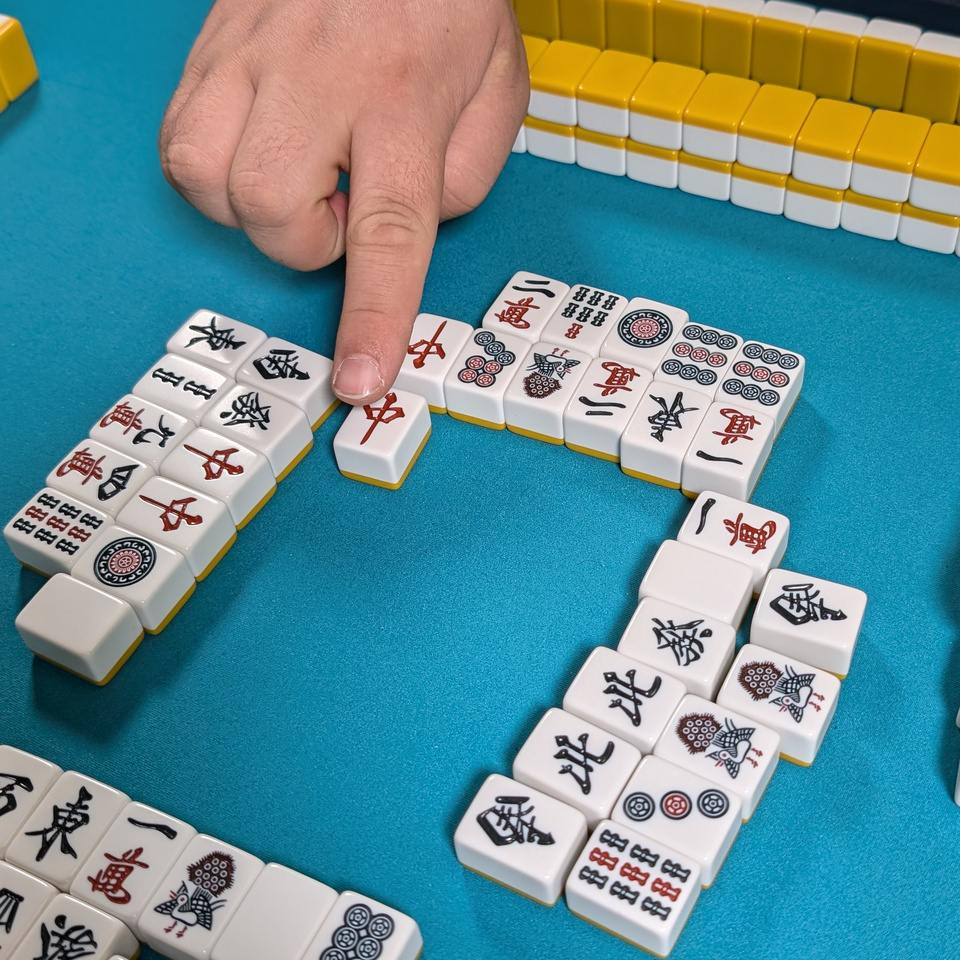
\includegraphics[width=8cm]{72_dont-play-with-discard.jpg}
	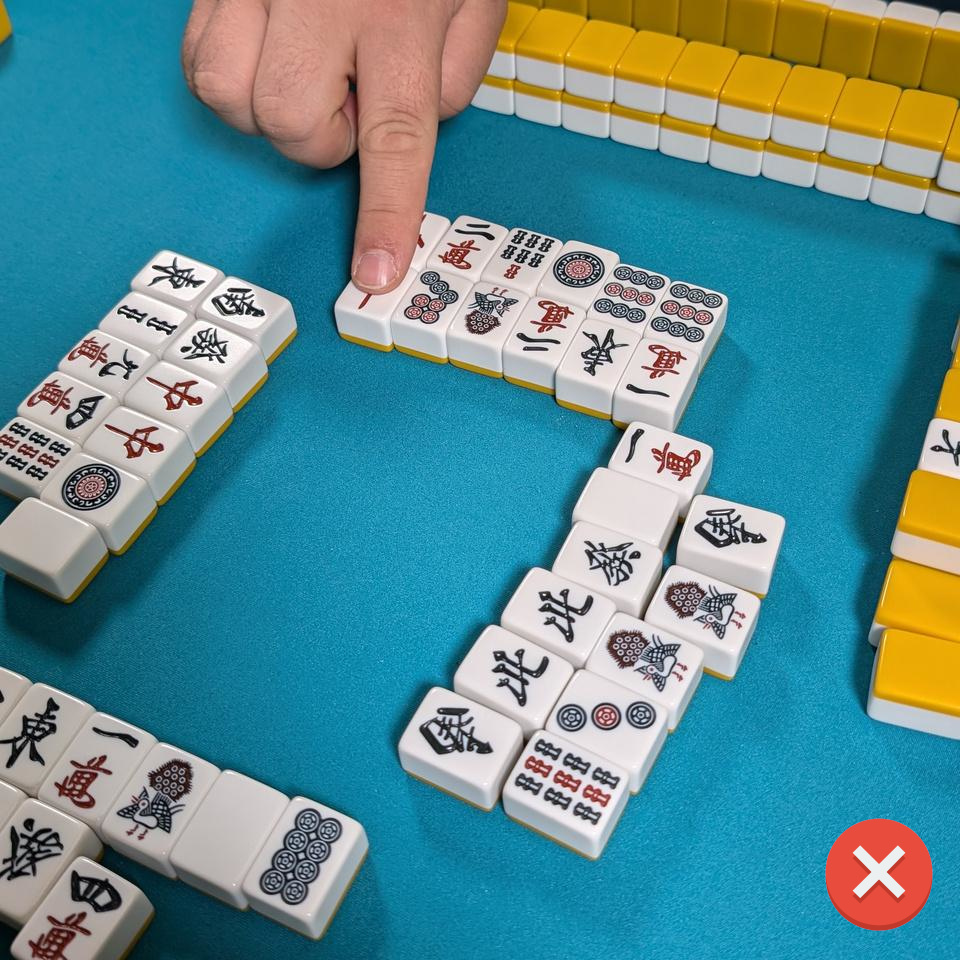
\includegraphics[width=8cm]{73_dont-play-with-discard.jpg}
	\caption{Не играйте с дискардом}
\end{figure}

Не трогайте чужие дискарды. Если дискард оппонента выглядит хаотично, вы вправе попросить его поправить дискард, но не делайте это самостоятельно. Единственный случай, когда вы вправе прикасаться к чужому дискарду --- это взятие тайла в сет.

\begin{figure}[H]
	\centering
	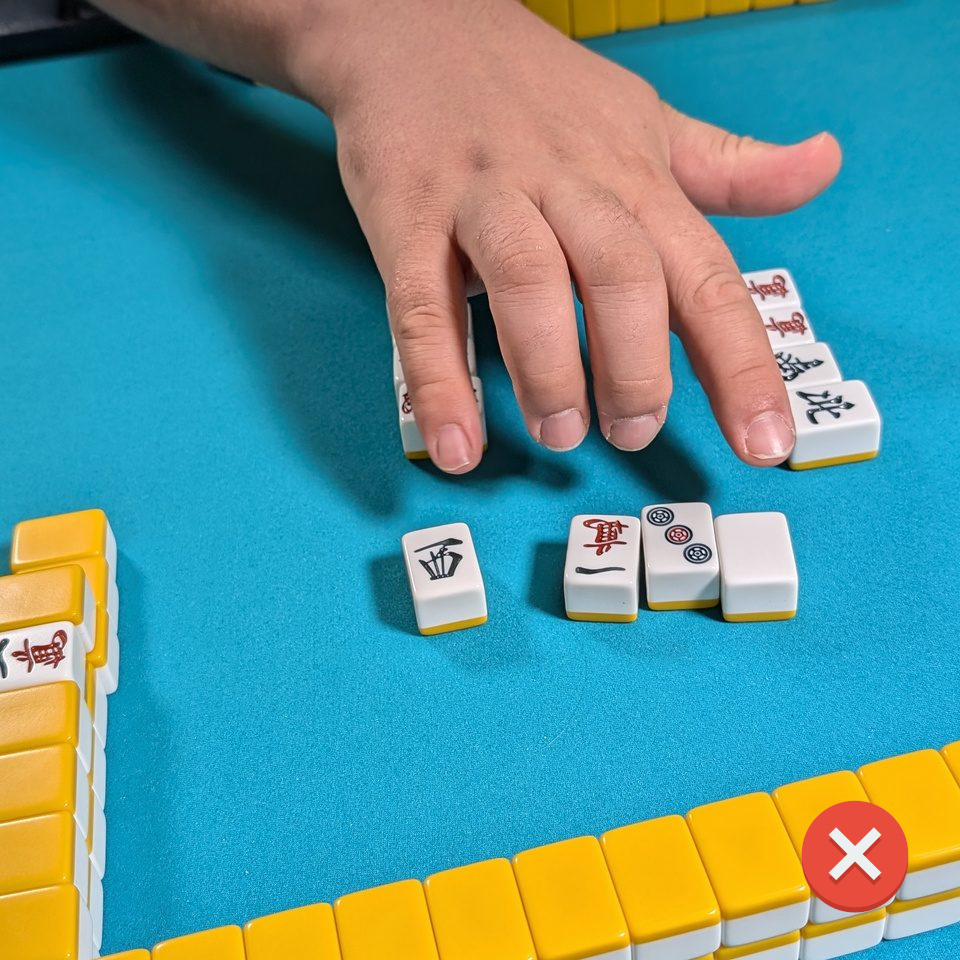
\includegraphics[width=8cm]{69_dont-touch-discards.jpg}
	\caption{Не трогайте чужие дискарды}
\end{figure}

Нельзя забрать только что сброшенный тайл обратно в руку и сбросить другой - при нарушении может быть объявлена мертвая рука.

На сброс в среднем дается несколько секунд. Допускается размышление в течение 10-15 секунд над некоторыми сбросами, однако если игрок намеренно затягивает игру, сбрасывая каждый тайл после длительного размышления, это может быть интерпретировано как препятствование ходу игры. В этом случае следует вызвать судью и зафиксировать нарушение.

\subsection{Объявления}

В случае объявления сета, игрок обязан делать объявление громко и четко. В случае, если игроку требуется некоторое время на раздумия, игрок вправе попросить оппонентов подождать перед следующим взятием, однако не следует злоупотреблять этим правом --- если игрок слишком часто просит подождать, это может быть воспринято как затягивание игры с последующим назначением штрафа за неспортивное поведение. Не рекомендуется размышлять над взятием более 5 секунд.

\subsubsection{Объявления понов и чи}

При объявлении пона с игроков справа или напротив, игроку следует стараться сделать объявление как можно быстрее, чтобы игрок, чей ход в данный момент, не успел взять и посмотреть тайл или не объявил чи. Если очевидно, что игрок не торопится сделать взятие и раздумывает над чи --- также следует объявить пон как можно раньше, чтобы игрок не открыл тайлы в своем сете. Если игрок успел сказать "чи", допустимо сказать "пон", но следует сделать это до того как игрок открыл два своих тайла. 

Некоторые игроки практикуют "пон вредности", используя правило приоритета объявления пона над объявлением чи (ситуация: объявление "пон" непосредственно после объявления "чи", сделанное по причине того, что оппонент решает объявить чи). Данную практику мы рассматриваем как дурной тон и не рекомендуем ее использовать исходя из принципов честной игры. Однако, поскольку невозможно точно определить, является ли объявление "поном вредности" или игрок просто задумался и сделал объявление с запозданием, запретить такие объявления мы не можем и оставляем их на совести игроков. Наказаний за "пон вредности" также не предусматривается из-за сложности доказательства намерения. Игроку, который хочет объявить чи, рекомендуется выждать пару секунд, убедившись что никто не планирует объявлять пон, и только потом делать объявление. В случае объявления пона во время паузы, ситуация разрешается обычным образом в пользу объявления пона.

После объявления (которое нужно сделать достаточно громко, убедившись что все услышали и никто не пытается взять следующий тайл и продолжить игру) следует последовательно открыть два тайла из руки, потом отложить их справа от руки, далее забрать объявленный тайл, потом сформировать сет, корректно повернув взятый тайл, чтобы он указывал на игрока, с которого он был взят, отложить сет в правый угол стола, и наконец произвести сброс.

\begin{figure}[H]
	\centering
	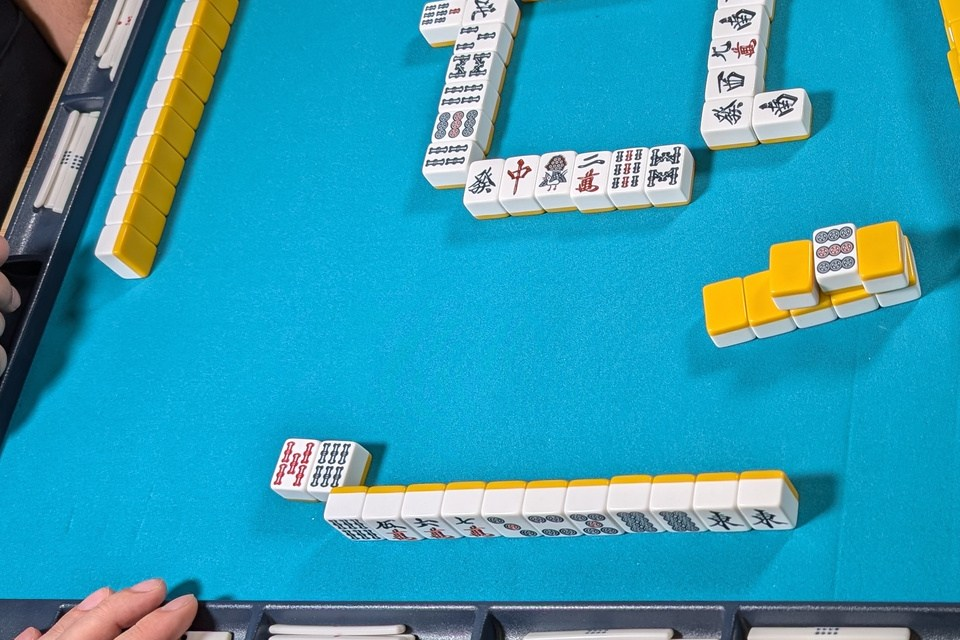
\includegraphics[width=8cm]{22_chi.jpg}
	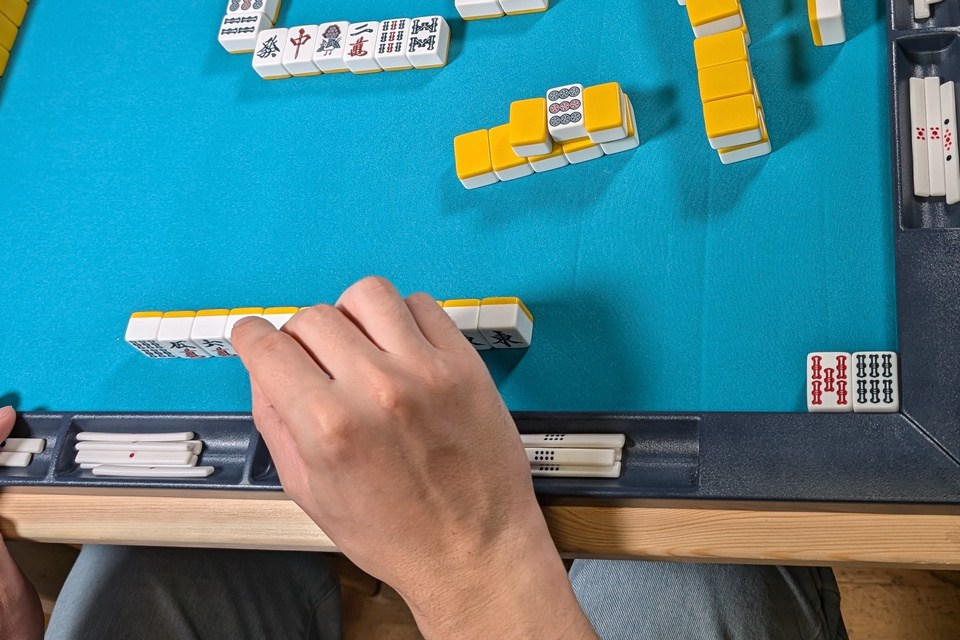
\includegraphics[width=8cm]{23_chi.jpg}
	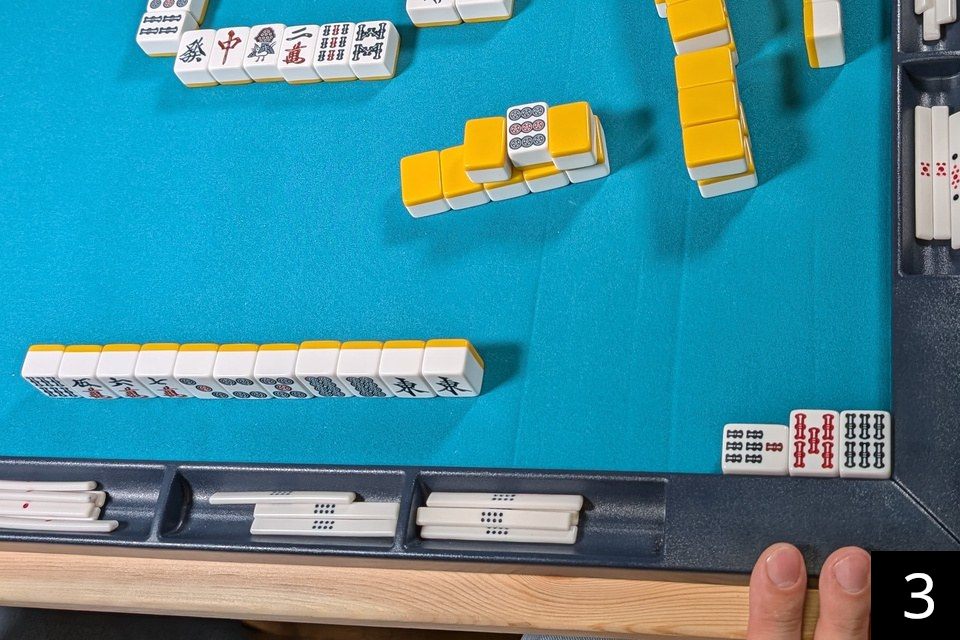
\includegraphics[width=8cm]{24_chi.jpg}
	\caption{Правильная последовательность объявления сета, после которой следует сброс}
\end{figure}

Допускается сначала сделать сброс, а затем забрать тайл из дискарда в сет. Рекомендуется это делать одним движением, чтобы дискард был виден для всех игроков максимальное количество времени. В случае, если на дискарде игрока, только что открывшего сет, делается еще одно объявление, следует подождать, пока игрок полностью завершит объявление и только после этого делать сброс и брать тайл из дискарда.

Некоторые игроки открывают сразу три тайла --- объявляемые и тот, который пойдет в дискард. Следует отказаться от этой практики, поскольку иногда по такому открытию неочевидно, какие именно тайлы мы объявляем, а какой готовимся сбросить (например если на сбросе 2 открыть 134). Если игрок еще не решил, что именно будет сбрасывать, следует сначала подумать, и открывать сет только после того как решение принято. Открытие трех тайлов сразу может наказываться вежливым указанием и штрафом в случае повторения.

В случае если игрок случайно открыл тайлы, которые не завершают сет, и это было быстро замечено им или указано на это другими игроками, необходимо либо открыть корректные тайлы, либо, если их в руке нет, отменить объявление. Такое поведение наказывается вежливым указанием так не делать, но может и повлечь за собой штраф в случае повторения ситуации.

В случае если никто не заметил некорректного объявления сразу, игра была продолжена, а ошибка была замечена впоследствии --- игроку назначают мертвую руку.

При объявлении нескольких сетов, можно выкладывать их в правом углу как справа налево, так и снизу вверх, но рекомендуется выкладывать именно снизу вверх, т.к. при трех и более объявлениях, когда тайлы выложены справа налево, мы будем перекрывать их видимость для других игроков при своем взятии из стены, а объявления должны быть всегда и всем видны. Не следует смешивать порядок --- например, класть второе объявление сверху над первым, а третье слева от него. Не следует класть более ранние объявления левее/выше более поздних, всегда должно быть однозначно видно, в каком порядке были сделаны объявления в раздаче.

\begin{figure}[H]
	\centering
	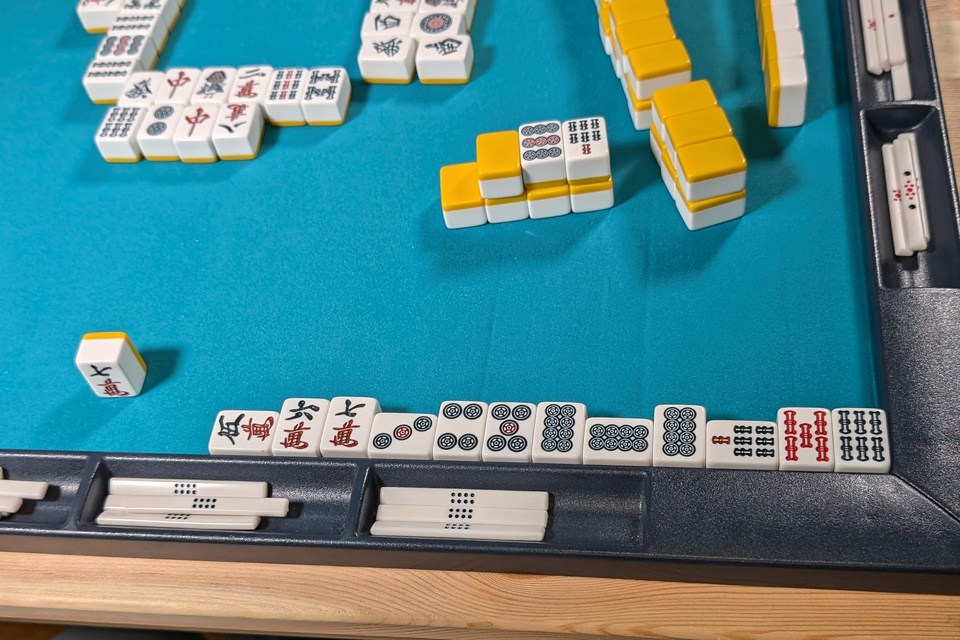
\includegraphics[width=8cm]{25_sets-position.jpg}
	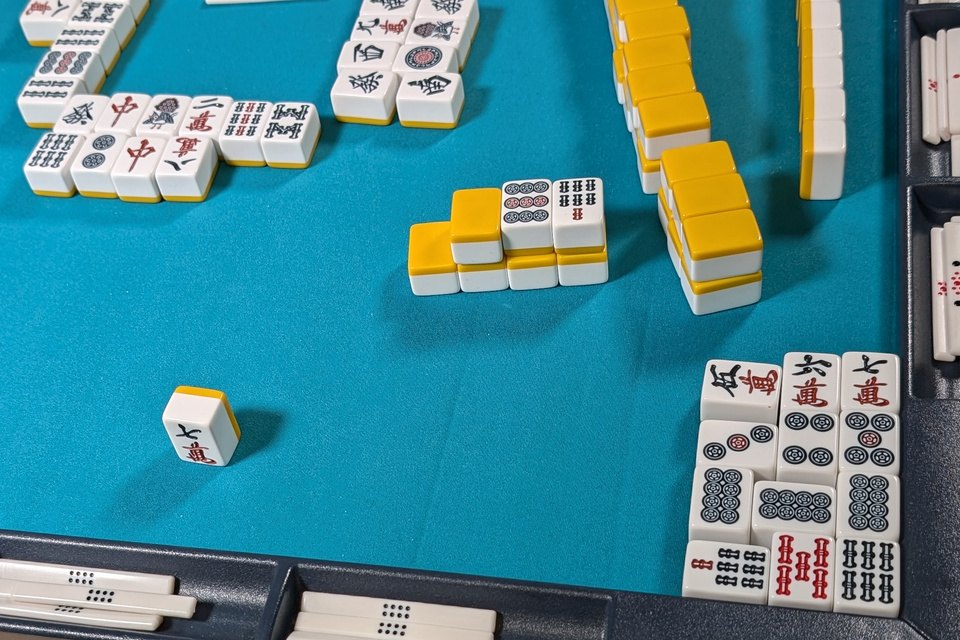
\includegraphics[width=8cm]{26_sets-position.jpg}
	\caption{Допустимый и рекомендуемый варианты размещения сетов}
\end{figure}

На последнем сбросе в раздаче никакие объявления, кроме объявления победы, недопустимы.

Недопустимо выкладывать сеты в левом углу или в середине руки. Это дезориентирует игроков и они вправе попросить так не делать, а если игрок не прислушивается к просьбе --- то и вызвать судью для вынесения вежливого указания или штрафа при повторении ситуации.

\begin{figure}[H]
	\centering
	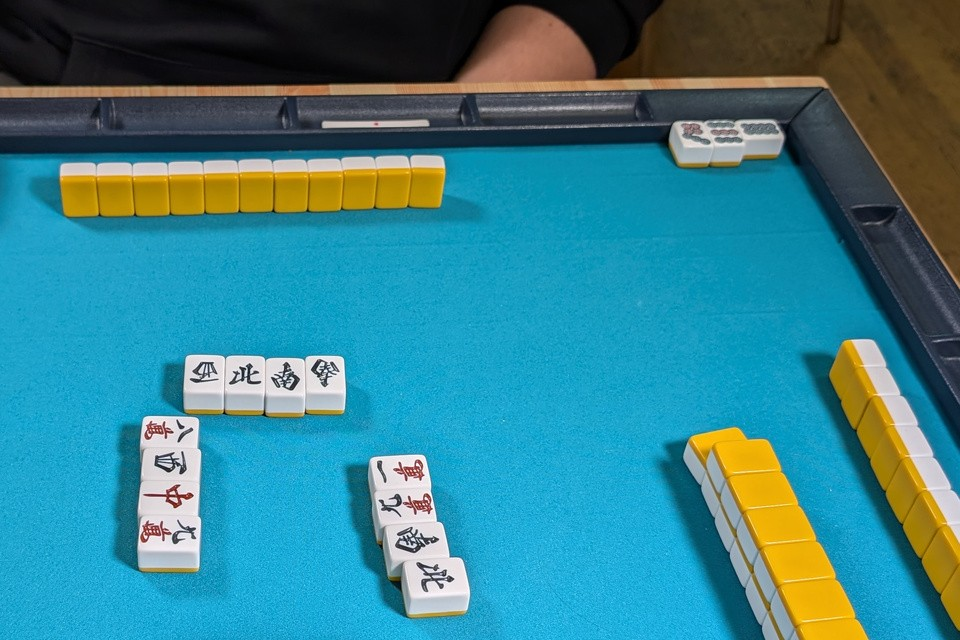
\includegraphics[width=8cm]{27_sets-position-wrong.jpg}
	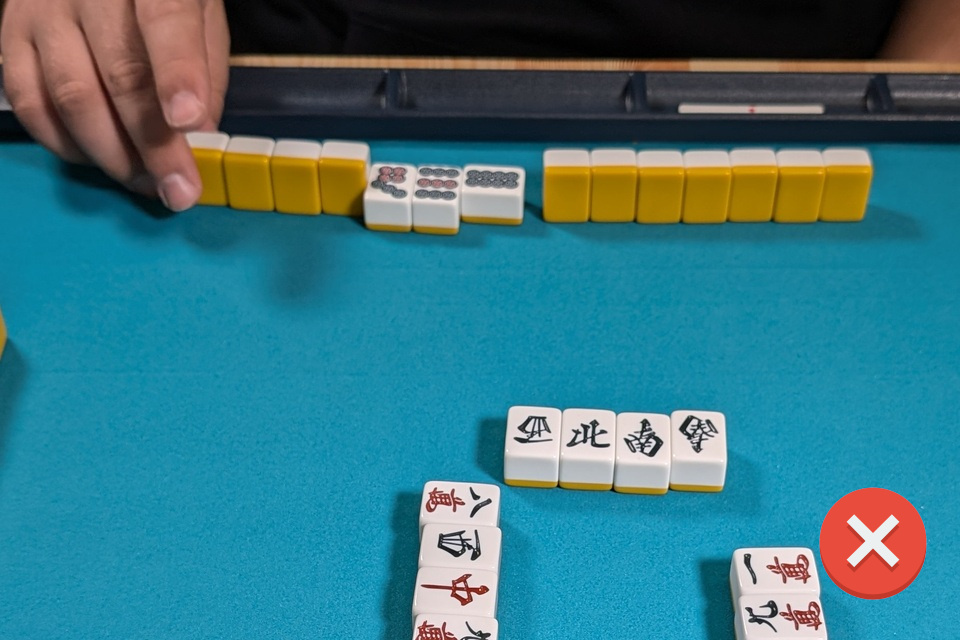
\includegraphics[width=8cm]{28_sets-position-wrong.jpg}
	\caption{Недопустимые варианты размещения сетов}
\end{figure}

\subsubsection{Объявление канов}

Открытие канов похоже на объявление понов --- последовательность действий при объявлении следует соблюдать аналогичным образом. Рассмотрим отличия, характерые именно для канов.

Закрытый кан или дополнение пона до кана возможны только после взятия из стены (живой или мертвой), нельзя объявить никакой кан сразу после объявления пона/чи.

После того как игрок объявил кан и показал корректно все 4 тайла (при закрытом кане), 3 тайла при открытом кане, 1 тайл при апгрейде пона до кана (если не был объявлен рон чанкан), игрок, с чьей стороны находится новый индикатор доры, сразу переворачивает его. Игрок, объявивший кан, сформировав его в правом углу, обязательно берет тайл замены, прежде чем сделать сброс. Допускается открывать новый индикатор после взятия тайла замены, но обязательно это сделать до сброса игрока, объявившего кан. Если игроки видят, что игрок готовится сбросить тайл слишком рано, они должны напомнить ему о необходимости взять тайл замены. Открытые индикаторы будут применяться в том числе при победе на тайле замены.

\begin{figure}[H]
	\centering
	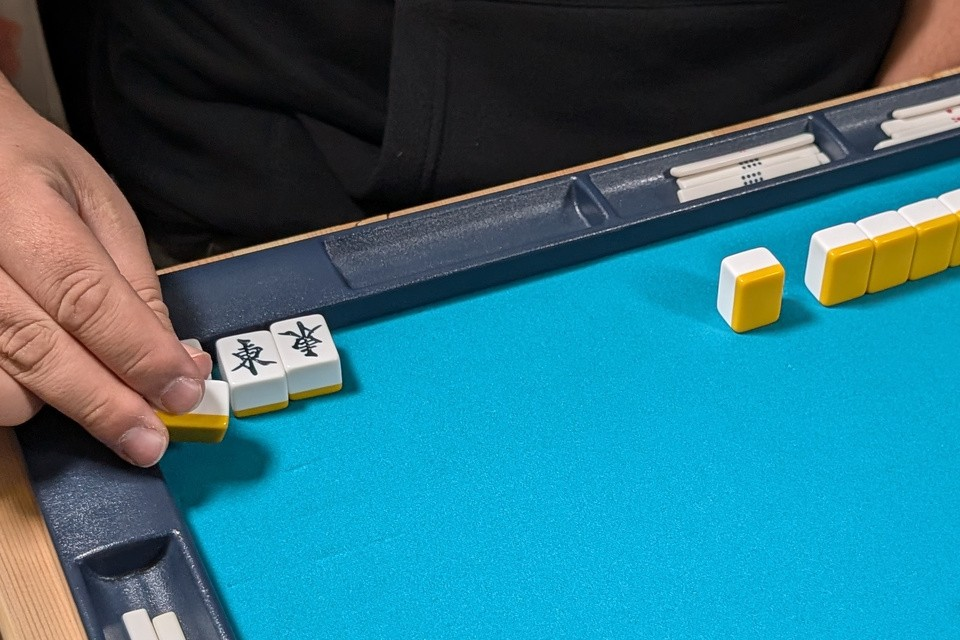
\includegraphics[width=8cm]{29_kan.jpg}
	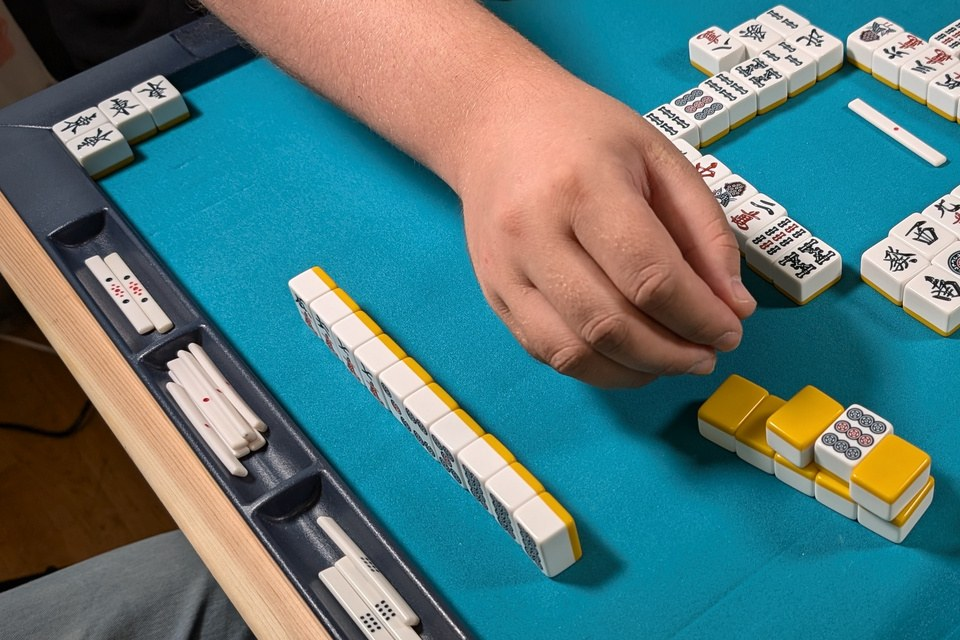
\includegraphics[width=8cm]{30_kan.jpg}
	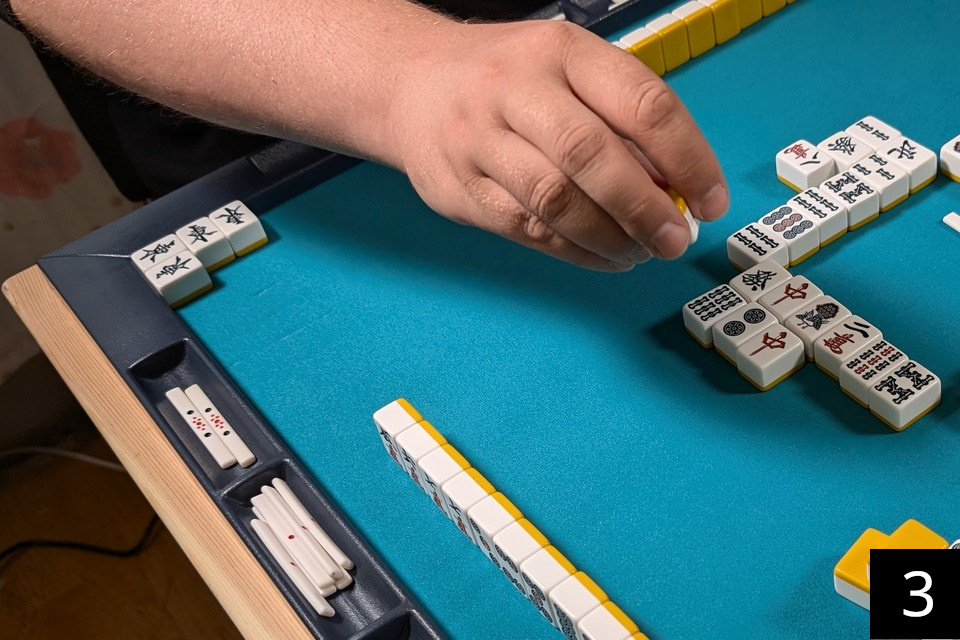
\includegraphics[width=8cm]{31_kan.jpg}
	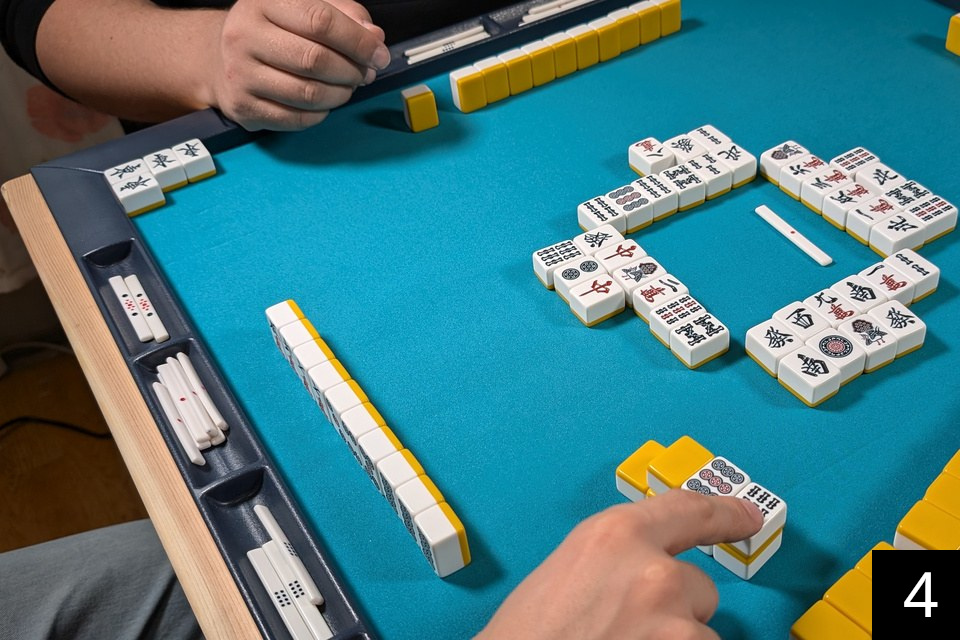
\includegraphics[width=8cm]{32_kan.jpg}
	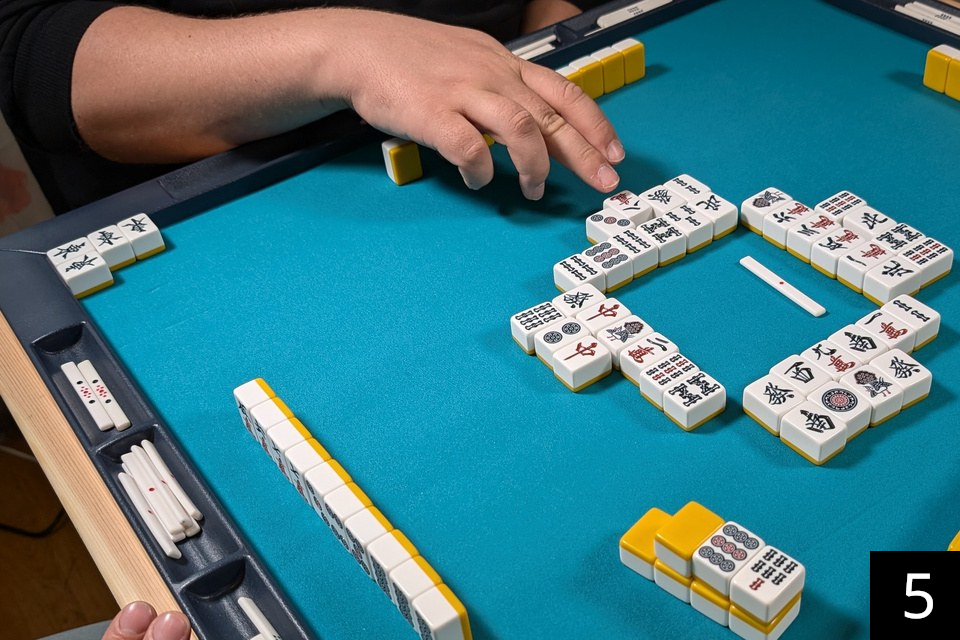
\includegraphics[width=8cm]{33_kan.jpg}
	\caption{Корректный порядок объявления кана}
\end{figure}

Нужно не забывать, что после того, как игрок объявил кан и взял тайл замены, живая стена стала на один тайл короче, т.к. в мертвой стене всегда должно быть 14 тайлов. Не рекомендуется делать каких-либо манипуляций с мертвой стеной, если до конца раздачи еще далеко --- это лишняя трата времени. Кроме того, можно запутаться и переместить в мертвую стену не тот тайл. В идеале, когда раздача будет близиться к концу, игрокам нужно прикинуть, какой тайл на данный момент будет последним, после чего можно слегка его подвинуть и указать всем условно что "последний тайл в раздаче вот этот". Если кто-то из игроков настаивает на снятии этого тайла для более простого восприятия --- игрок, в чьей стене на данный момент находится последний тайл, аккуратно его перемещает в конец живой стены, и все следят, чтобы ничего не было перепутано.

\begin{figure}[H]
	\centering
	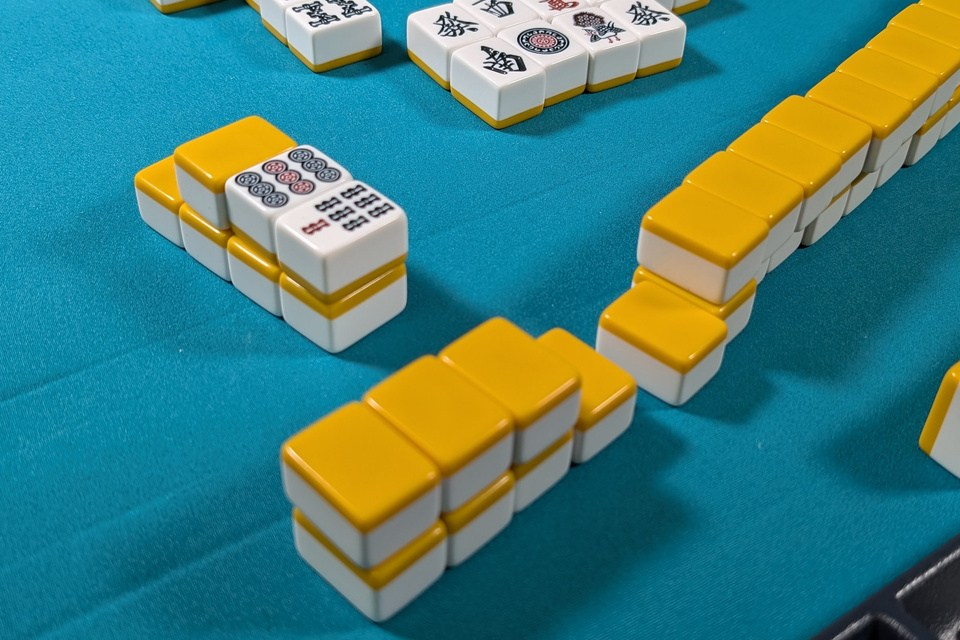
\includegraphics[width=8cm]{34_kan-walls.jpg}
	\caption{Перемещение последнего тайла живой стены в мертвую}
\end{figure}

Также кратко стоит упомянуть важный момент --- кан можно объявить только если в живой стене есть хотя бы один тайл --- т.к. этот тайл нужно переместить в мертвую стену (а если тайлов в живой стене нет --- то перемещать нечего). При этом последнее взятие в игре будет из мертвой стены, в случае победы на нем будет засчитан риншан, но не хайтей (риншан и хайтей не сочетаются). При объявлении закрытого кана пятерок при игре с акадорами --- красная пятерка должна быть среди видимых, чтобы при подсчете стоимости руки ее не забыли посчитать.

\subsubsection{Объявление риичи}

Крайне важно соблюдать корректный порядок объявления: 
\begin{itemize}
	\item Громко (чтобы все услышали и обратили внимание) сказать "риичи";
	\item Сбросить тайл боком в дискард
	\item Убедиться, что на сброшенном тайле не объявлена победа
	\item Положить ставку риичи перед дискардом.
\end{itemize}

\begin{figure}[H]
	\centering
	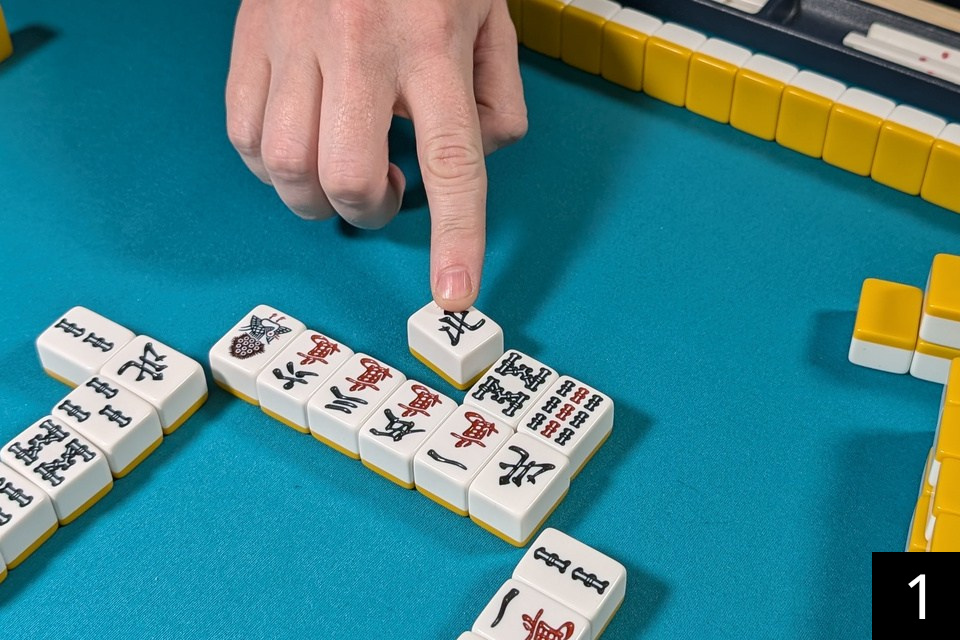
\includegraphics[width=8cm]{35_riichi.jpg}
	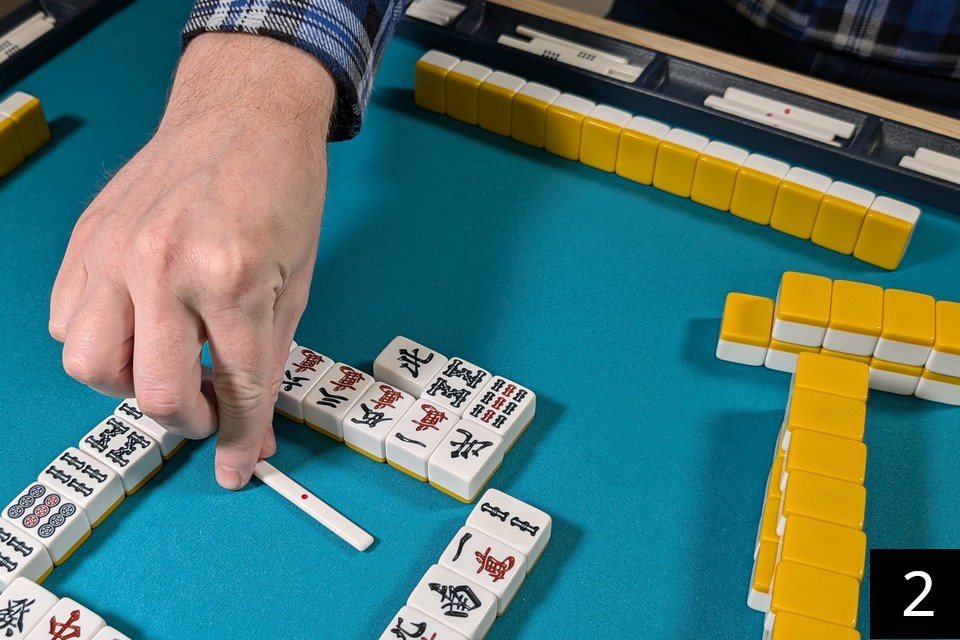
\includegraphics[width=8cm]{36_riichi.jpg}
	\caption{Объявление риичи}
\end{figure}

\newpage

Не следует кидать риичи-палочку в центр стола. Место риичи-палочки --- зона непосредственно перед вашим дискардом. 

\begin{figure}[H]
	\centering
	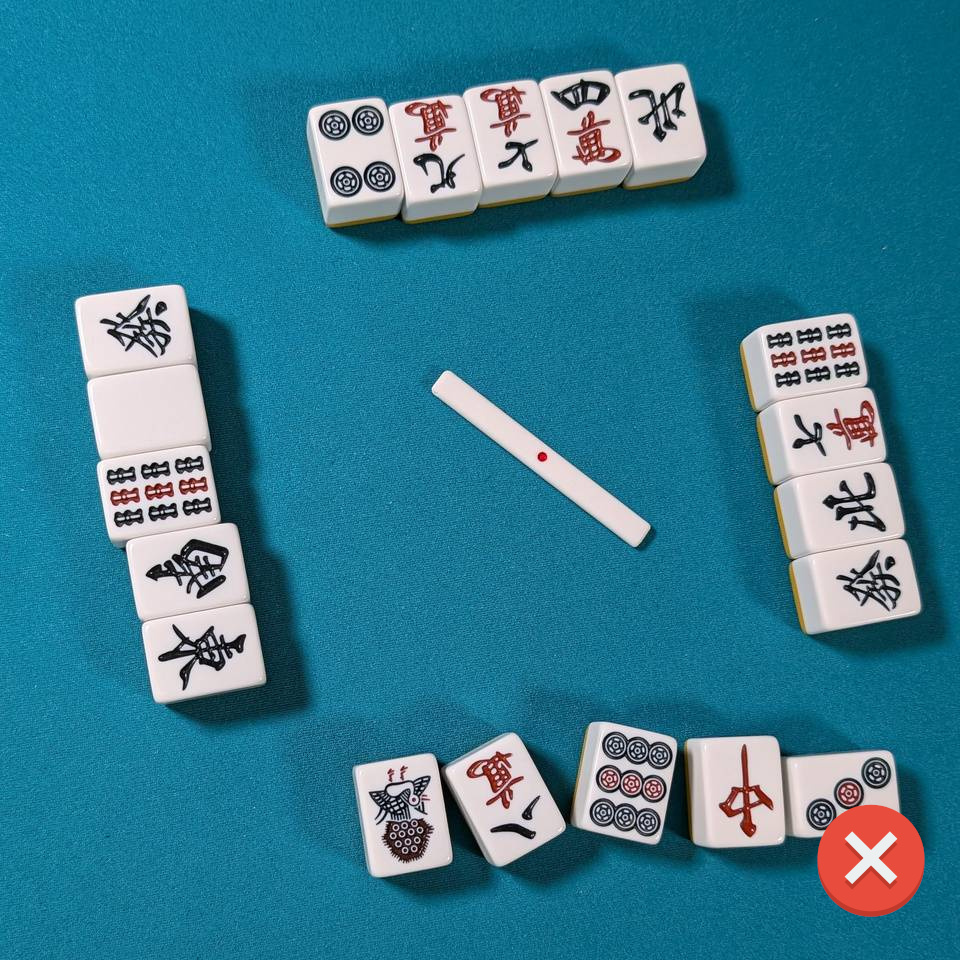
\includegraphics[width=8cm]{66_chaotic-riichi.jpg}
	\caption{Не делайте так}
\end{figure}

Если тайл был взят в любой сет --- нужно не забыть повернуть свой следующий сброшенный тайл (если забыли --- сразу, как только ошибка была обнаружена, всем столом восстановить последовательность и повернуть правильный тайл). Некорректный порядок объявления риичи приводит к тому, что объявление не засчитывается. Не допускается объявлять риичи после сброса (ситуация "никому не нужно? тогда риичи"), такое риичи также не засчитывается, а за пустое объявление назначается вежливое указание так не делать, а при повторении --- штраф. Также не следует класть сброс для риичи рядом с рукой, поскольку такое действие может быть расценено как объявление победы по цумо.

\begin{figure}[H]
	\centering
	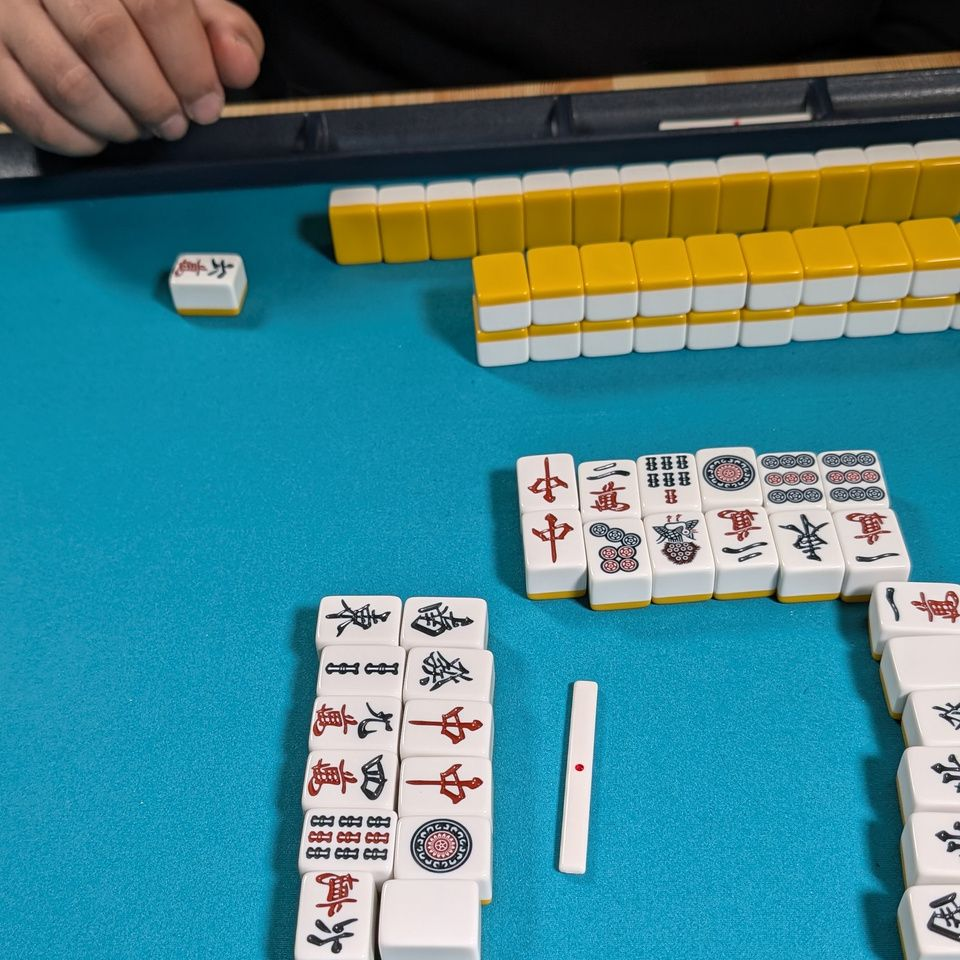
\includegraphics[width=8cm]{37_discard-riichi-tile-directly.jpg}
	\caption{Некорректное объявление риичи}
\end{figure}

Игрок справа перед своим следующим взятием должен дождаться, пока мы выполним все действия (повернем тайл, положим палочку), и только после этого делать взятие, то же касается игроков, которые хотят на нашем тайле сделать объявление --- можно сказать "пон"/"кан", но прежде чем забирать тайл они должны дождаться, пока игрок с риичи положит палочку. При объявлении победы ждать не требуется, т.к. палочку игрок в этом случае не кладет, победу нужно объявлять сразу.

После объявления риичи игроку не следует касаться взятым из стены тайлом своей руки, чтобы избежать подозрений в изменении руки. Взятые тайлы можно смотреть, не ставя тайл в руку, также допустимо ставить рядом с рукой (справа для правшей, слева для левшей), но не касаясь ее. В случае игры на трансляции, допускается положить взятый тайл боком на руку сверху --- это позволит зрителям видеть все взятые тайлы. Не следует класть невыигрышные тайлы лицевой стороной вверх рядом с рукой. Если тайл невыигрышный, открывать его нужно именно в дискарде, чтобы игроки не подумали, что вы объявляете победу --- за подобное расположение тайла полагается вежливое указание так не делать, а в случае повторения может быть назначен штраф.

Игрок, объявивший риичи, может объявить закрытый кан, в этом случае он сначала говорит "кан", потом кладет взятый тайл лицевой стороной вверх рядом с рукой и дополняет его тремя тайлами из руки, чтобы сформировать кан.

В случае ничьей, игроки, объявившие риичи, обязательно показывают состояние своей руки, чтобы все могли убедиться, что у них есть темпай, даже если после риичи игроку по каким-то причинам была объявлена мертвая рука (например при некорректном объявлении победы). Игрок с мертвой рукой будет считаться нотен, показ руки необходим, чтобы убедиться, что риичи было корректно (в руке был темпай), а также что после риичи не было некорректных объявлений канов. В случае нарушения, игрок получает чомбо.

Риичи можно объявить только если в живой стене осталось не меньше четырех тайлов (если при отсутствии каких либо объявлений у объявляющего риичи игрока будет хотя бы одно взятие). 

\newpage

Некоторые игроки приносят на турниры и на клубные игры собственные риичи-палочки, которые выглядят нестандартным образом (например, похожие на различные риичи-палочки на платформе MahjongSoul). Игрок может использовать нестандартную риичи-палочку в случае соблюдения следующих условий:

\begin{itemize}
	\item Турнир проводится с использование системы автоматизированного подсчета очков (т.е. в исходном наборе у каждого игрока только одна палочка номиналом в 1000 очков).
	\item Организаторами турнира разрешено использование в данном турнире нестандартных риичи-палочек.
	\item Игрок получил согласие главного судьи турнира на использование конкретной нестандартной риичи-палочки.
	\item Игрок перед началом каждого ханчана в явном виде спросил у своих оппонентов, не против ли они использования его конкретной нестандартной риичи-палочки и получил их согласие.
	\item Игрок располагает нестандартную риичи-палочку перед собой (в лотке мата или же, при использовании других вариантов игрового покрытия, там же, где остальные игроки держат свои риичи-палочки).
\end{itemize}

Если любое из указанных условий не соблюдается, это ведет к запрету на дальнейшее использование им нестандартной риичи-палочки в рамках данного турнира. Главному судье турнира рекомендуется не одобрять для использования риичи-палочки, изображающие неуместные или вызывающие предметы, а также палочки, которые плохо видны на поверхности стола. Любые посторонние предметы недопустимо использовать в качестве риичи-палочек. Если риичи-палочка допущена до игры, игроку следует убрать стандартную (предоставленную организаторами турнира) риичи-палочку из поля зрения всех игроков, а после окончания ханчана возвращает ее на место (в лоток джанк-мата или на стол).

\begin{figure}[H]
	\centering
	\includegraphics[width=8cm]{38_no-custom-sticks.jpg}
	\caption{Посторонний предмет в качестве риичи-палочки}
\end{figure}

\subsection{Победа и ничья}

\subsubsection{Объявление победы}

При объявлении победы с дискарда следует соблюдать корректный порядок действий:

\begin{itemize}
	\item Объявить "рон" достаточно громко, чтобы все услышали, и убедиться что никто не пытается продолжить игру, взяв тайл из стены или объявив пон на том же тайле;
	\item Осторожно открыть всю руку;
	\item В случае победы с риичи --- открыть и показать всем урадоры;
	\item Перечислить все комбинации в руке, назвать общее количество дор и итоговое количество хан и фу.
\end{itemize}

\newpage

Рекомендуется также отделить тайлы, формирующие ожидание, для упрощения прочтения руки другими игроками.

\begin{figure}[H]
	\centering
	\includegraphics[width=8cm]{39_declare-ron.jpg}
	\includegraphics[width=8cm]{40_declare-ron.jpg}
	\caption{Объявление рона}
\end{figure}

Не разрешается забирать выигрышный тайл из сброса другого игрока. При нарушении может быть назначение вежливое указание (при повторном нарушении --- штраф). Обоснование заключается в том, что набросивший игрок может оспорить необходимость платить вам, т.к. в его сбросе нет вашего выигрышного тайла. Кроме того, возможны случаи, когда тайл наброшен в две и более рук. Если наброс произведен дорой, следует не забыть посчитать ее при перечислении количества дор в руке.

\begin{figure}[H]
	\centering
	\includegraphics[width=8cm]{43_declaring-ron-wrong.jpg}
	\includegraphics[width=8cm]{44_declaring-ron-wrong.jpg}
	\caption{Недопустимо забирать выигрышный тайл из дискарда}
\end{figure}

В случае выигрыша со стены также придерживаемся строгой последовательности:

\begin{itemize}
	\item Объявить "цумо" достаточно громко, чтобы все услышали, и убедиться что никто не пытается продолжить игру;
	\item Положить победный тайл сбоку от руки на некотором расстоянии. Встраивать тайл в руку не следует. Допускается сначала положить победный тайл сбоку от руки и немедленно громко объявить "цумо";
	\item Осторожно открыть всю руку;
	\item В случае победы с риичи --- открыть и показать всем урадоры;
	\item Перечислить все комбинации в руке, назвать общее количество дор и итоговое количество хан и фу.
\end{itemize}

\begin{figure}[H]
	\centering
	\includegraphics[width=8cm]{45_declaring-tsumo.jpg}
	\includegraphics[width=8cm]{46_declaring-tsumo.jpg}
	\caption{Объявление цумо}
\end{figure}

Не следует класть победный тайл перед рукой, особенно если стена перед вами полностью разобрана --- другими игроками это может быть воспринято как сброс, на нем могут попытаться объявить победу.

\begin{figure}[H]
	\centering
	\includegraphics[width=8cm]{48_declaring-tsumo-wrong.jpg}
	\includegraphics[width=8cm]{49_declaring-tsumo-wrong.jpg}
	\caption{Тайл перед рукой}
\end{figure}

В случае если игрок пытается объявить цумо положив тайл в области руки, но не сбоку от нее, ему следует вынести вежливое указание так не делать, но руку засчитать. 

\newpage

Не следует встраивать тайл в руку при объявлении цумо или приставлять тайл к руке. В общем случае такое действие является нарушением и как результат игроку не будут засчитаны яку, связанные с ожиданием (пинфу) и миниочки за ожидания. В отдельных случаях судья может засчитать очки за ожидание, если оно находится в другой части руки и тайл с краю явно не связан с тайлами около него, однако рекомендуется не допускать таких ситуаций.

\begin{figure}[H]
	\centering
	\includegraphics[width=8cm]{50_declaring-tsumo-wrong.jpg}
	\caption{Встраивание тайла в руку}
\end{figure}

При победе с риичи, выигравший игрок также должен показать всему столу урадоры. Допускается также попросить об этом игрока, рядом с которым находится мертвая стена. Индикаторы доры и урадоры рекомендуется размещать рядом с мертвой стеной. Допускается также выложить индикаторы лицевой стороной вверх в центр стола.

\begin{figure}[H]
	\centering
	\includegraphics[width=8cm]{41_ron-after-riichi.jpg}
	\includegraphics[width=8cm]{42_ron-after-riichi.jpg}
	\caption{Вскрытие урадоры}
\end{figure}

\begin{figure}[H]
	\centering
	\includegraphics[width=8cm]{60_indicators-in-center.jpg}
	\caption{Допускается выложить индикаторы в центре стола после победы}
\end{figure}

В случае, если игрок забыл перевернуть индикатор урадоры, следует перевернуть его и учесть количество урадор. Если мертвая стена уже была разрушена, а результаты внесены, перерасчеты не допускаются.

На момент открытия (независимо от того, произошел ли рон или цумо) рука должна быть отсортирована. В случае если игрок играет с неотсортированной рукой, допускается отсортировать руку непосредственно перед открытием или сразу же после открытия. При победе следует также позаботиться о том, чтобы все ожидания в руке были очевидны, в случае сложного ожидания - рекомендуется озвучить его.

\begin{figure}[H]
	\centering
	\includegraphics[width=8cm]{47_unsorted-tiles.jpg}
	\caption{\centering Неотсортированная рука при победе \linebreak должна быть отсортирована до объявления выплат}
\end{figure}

После объявления стоимости руки, нужно не забыть упомянуть про хонбу, если она есть, и по возможности назвать итоговую стоимость с учетом хонбы ("семь семьсот, с учетом двух хонб --- восемь триста" или "семьсот, тысяча триста, одна хонба, итого, восемьсот, тысяча четыреста").

Объявление стоимости при цумо следует начинать с меньшего значения во избежание путаницы (сравните --- "2 хан, 30 фу, пятьсот, тысяча" и "2 хан, 30 фу, тысяча пятьсот").

Объявление количества дор и якухаев рекомендуется делать максимально явным образом, например "якухай три, дора три", или "три доры, три якухая". Не рекомендуется использовать числовые обозначения для дор без упоминания слова "дора" (например, "тан-яо, три" и особенно "якухай, три" --- во избежание путаницы).

При объявлении победы, все игроки за столом имеют право проверить выигрышную руку на корректность (правильную форму, наличие яку, отсутствие фуритена). Победивший игрок не имеет права препятствовать подобным проверкам.

Не следует смотреть тайлы в стене после победы. Если победа была без риичи, не следует смотреть урадоры и тайлы замены. 

\begin{figure}[H]
	\centering
	\includegraphics[width=8cm]{76_no-wall-look.jpg}
	\caption{Не подсматривайте тайлы}
\end{figure}

\newpage

\subsubsection{Ничья}

При ничьей игроки показывают свой темпай. В случае если у игрока нотен, игрок должен закрыть руку или часть руки. Любое действие игрока, отличное от полного показа руки, трактуется как нотен. Рекомендуется также озвучивать состояние руки словами "темпай" и "нотен" для исключения двусмысленности.

Если игрок не объявлял риичи, он не обязан показывать руку, может объявить нотен и закрыть ее, даже если его рука открыта до одного тайла\footnote{Это может быть истиной, например при ожидании в тайл, пон которого уже открыт у игрока, но даже если это не так --- игрок в любом случае вправе закрыть руку, объявив нотен}. Объявление темпаев/нотенов следует производить поочередно, начиная с дилера (затем юг, запад, север). Открытие руки вне очереди не рекомендуется, но и не наказывается, при этом игрок имеет право не показывать состояние своей руки, пока игроки до него не покажут свое. В случае, если игрок показал темпай или нотен вне очереди, он не может поменять решение.

\begin{figure}[H]
	\centering
	\includegraphics[width=8cm]{51_declare-draw-start-from-dealer.jpg}
	\caption{Дилер объявил темпай первым}
\end{figure}

Дилеру может быть выгодно показать нотен, если у определенных игроков тоже нотен (например, чтобы завершить игру), но другие игроки не обязаны раскрывать ему состояние руки, пока он не объявит свое.

\subsubsection{Расчеты за победу/ничью}

После того, как победивший игрок назвал стоимость своей руки, игроки, которые делают выплаты, должны положить соответствующую сумму на стол рядом с собой. Не следует класть палочки поближе к выигравшему --- в случае цумо, когда так сделают несколько игроков, будет непонятно кто сколько положил. При расчетах следует стремиться к тому, чтобы было использовано как можно меньше палочек --- при победе в 3900 следует дать пятитысячную палочку и попросить сдачу в тысячу сто. По возможности, размен стоит производить палочками, которые уже лежат на столе, например если игрок собрал по цумо 700/1300, дилер может дать две тысячных палочки и забрать в качестве сдачи 700 очков, которые дал другой игрок, но подобные действия при расчете следует озвучивать вслух. В случае, если на столе были риичи-палочки --- победившему игроку (а в случае дабл-рона --- имеющему на них право игроку), следует сразу подвинуть их к себе, чтобы они не смешивались с очками, которыми будут производиться выплаты. Также после выплат игрокам стоит убедиться, что у них есть хотя бы одна тысячная палочка для объявления риичи, и в случае ее отсутствия попросить у других игроков размен.

\begin{figure}[H]
	\centering
	\includegraphics[width=8cm]{53_points-pass.jpg}
	\caption{Расчет палочками}
\end{figure}

В случае, если при объявлении риичи обнаружилось, что тысячной палочки нет --- также стоит попросить размен, желательно непосредственно перед объявлением риичи, а не в момент, когда кладется палочка, как на картинке выше.

Не допускается начинать замешивание тайлов до того, как все выплаты были учтены.

\begin{figure}[H]
	\centering
	\includegraphics[width=8cm]{77_no-messing.jpg}
	\caption{Замешивание тайлов до окончания расчетов}
\end{figure}

Только после того, как очки были проверены всеми игроками и учтены, допускается перевернуть тайлы и приступить к перемешиванию тайлов, любые изменения в расчетах после этого момента производиться не должны. Если все за столом согласны, например игроки вспомнили, что забыли отметить чью-то риичи-палочку, или недосчитали дору, допустим перерасчет, но только если все игроки за столом действительно помнят, что было именно так, и не против внести изменения.

\newpage

\subsection{Поведение за столом и внешний вид}

Следует обратить внимание на то, как вы сидите: не скрещивайте руки, не кладите ногу на ногу, не ставьте локти на стол и не подпирайте голову рукой. Не держите обе руки на тайлах своей руки.

\begin{figure}[H]
	\centering
	\includegraphics[width=8cm]{54_pose.jpg}
	\includegraphics[width=8cm]{55_pose.jpg}
	\includegraphics[width=8cm]{56_pose.jpg}
	\caption{Плохие варианты поз за игровым столом}
\end{figure}

\newpage

Держаться следует свободно, открыто, расслабленно, нерабочую руку (для праворуких — левую и наоборот) желательно класть на колено.

\begin{figure}[H]
	\centering
	\includegraphics[width=8cm]{57_pose-good.jpg}
	\caption{Правильная поза за столом}
\end{figure}

Не следует закрывать свою руку в процессе игры, в частности --- не следует закрывать руку после объявления риичи. Если рука была закрыта, другие игроки могут счесть вашу руку за часть стены и сделать взятие из нее --- в этом случае вы сами будете виноваты в том, что ваша рука признана мертвой.

\begin{figure}[H]
	\centering
	\includegraphics[width=8cm]{58_close-hand-wrong.jpg}
	\caption{Рука при риичи}
\end{figure}

\newpage

Не рекомендуется (но не наказывается) закрытие единственного тайла в руке.

\begin{figure}[H]
	\centering
	\includegraphics[width=8cm]{59_close-hand.jpg}
	\caption{Один оставшийся тайл в руке}
\end{figure}

Повторим также еще раз --- необходимо делать все объявления громко и четко, несоблюдение этого правила может быть наказано вежливым указанием или штрафом в случае повторения.

Игроки, чей внешний вид отвлекает от игры, могут быть отстранены от турнира по решению судьи. Не допускаются вызывающие костюмы, маски. Помните, что турнир - это не маскарад и не пространство для самовыражения.

Не допускается использование мобильных устройств за столом (за исключением случая внесения раздачи или просмотра состояния стола). Общение в мессенджерах и звонки по телефону наказываются штрафом от 8000 очков на усмотрение судьи. В случае, если игрок ожидает важного звонка, он обязан предупредить об этом судью и оппонентов. На время разговора игрок должен выйти из-за стола и из игрового зала.

\begin{figure}[H]
	\centering
	\includegraphics[width=8cm]{61_texting.jpg}
	\caption{Не отвлекайтесь от игры}
\end{figure}
